\documentclass[a4paper,12pt]{article}
\usepackage[latin1]{inputenc}
\usepackage[italian]{babel}
\usepackage{graphicx}
\usepackage{listings}
\usepackage{fancyhdr}
\usepackage{multicol}
\usepackage[pdftex]{color}
\usepackage{url}
\usepackage[final]{pdfpages}
\newcommand{\fncyblank }{\fancyhf {}}

\definecolor{Gray}{cmyk}{0,0,0,0.50}

\lstset{language=C}
\lstset{frame=trBL}
\lstset{tabsize=1,breaklines,commentstyle=\textit}
\lstset{showstringspaces=false}
\lstset{basicstyle=\footnotesize}
\lstset{emph={},emphstyle=\textit}

\renewcommand{\lstlistingname}{Listato}
\renewcommand{\lstlistlistingname}{Elenco dei listati}

\newcommand{\cfile}[1]{\mbox{``\textit{#1}''}}
\newcommand{\ccode}[1]{\mbox{\textit{#1}}}

\addtolength{\hoffset}{-1cm}
\addtolength{\textwidth}{2cm}
\addtolength{\voffset}{-1cm}
\addtolength{\textheight}{1cm}

%AMBIENTE PER LO PSEUDOCODICE
\lstnewenvironment{pseudo}[2] {\lstset{ %
    language=C++, % choose the language of the code
%basicstyle=\footnotesize,       % the size of the fonts that are used for the code
%numbers=right,                   % where to put the line-numbers
numberstyle=\footnotesize,      % the size of the fonts that are used for the line-numbers
%stepnumber=1,                   % the step between two line-numbers. If it's 1 each line will be numbered
numbersep=1pt,                  % how far the line-numbers are from the code
backgroundcolor=\color{white},  % choose the background color. You must add \usepackage{color}
showspaces=false,               % show spaces adding particular underscores
showstringspaces=false,         % underline spaces within strings
showtabs=false,                 % show tabs within strings adding particular underscores
frame=single,                   % adds a frame around the code
frame=shadowbox
tabsize=2,                      % sets default tabsize to 2 spaces
captionpos=b,                   % sets the caption-position to bottom
breaklines=true,                % sets automatic line breaking
breakatwhitespace=true,        % sets if automatic breaks should only happen at whitespace
escapeinside={(*@}{@*)},          % if you want to add a comment within your code
%MIEI =P
mathescape=true,
columns=flexible,
morekeywords={for,forall},
#1,
label={code:#2}
}}{}

\title{System Paradigms and Models Project}
\author{Andrea Lottarini, Alberto Bandettini}
\date{September, 27 2010}

\begin{document}
\maketitle
\tableofcontents
\section{Introduction}  

In this section we will briefly introduce the aim of this project and the algorithm that we studied and implemented in a parallel fashion.
The algorithm is the Gauss-Newton algorithm for non linear least square interpolation.
In this particular case we studied an implementation of the algorithm for three dimensional interpolation of images representing gaussian beams.
The sequential version of the algorithm was developed in summer 2009 for interpolation of images of laser beams monitored by digital camera. 
By interpolation it is possible to monitor the output of a high definition camera with a precision down to micrometers, this operation requires lots of computation nonetheless.
This constitute the main reason for a parallel version of the program.

\subsection{Experimental Setup}

In this section we will briefly illustrate the environment where the algorithm is used and the main purpose for its development.
Laser beams are used to monitor the position and orientation of suspended mirrors used in the interferometer. 
The beam is pointed towards the mirror with a 45 degree angle and reflected on the screen of a high resolution digital camera.
Tilting of the mirror will produce a movement in the position of the laser beam while distortion of the surface of the mirror will produce a change in focus (size) of the beam.
Using then multiple cameras is possible to have a complete three dimensional displacement of the mirror in real time.
In order to do so position and size of the beam should be monitored with high precision. 
As said before the best way to do so is to interpolate the profile of the captured image of the laser beam which, in normal operative conditions, have a perfect gaussian shape.
Since the output of the camera is used for adjustments on remote controlled machinery it is important to have both a high throughput in terms of number of images elaborated and high precision of the interpolation itself.
In our opinion this was a nice real life case for studying parallelism.
Now let's analyse the algorithm used for interpolation.

\subsection{Algorithm}

The algorithm is the well known Gauss-Newton algorithm for non linear least square problems.
As the name says this algorithm does not perform perfect interpolation but tries to reduce as most the square error.
It is also applied for a non linear function (gaussian).
Linear methods as polynomial interpolation can be solved in a single step operating on every point (pixel) only once, non linear methods are iterative and so tends to converge after a  number of steps.
The pseudo code of the algorithm is shown in Figure \ref{code:gauss}.

\begin{figure}[h]
\begin{center} 
\begin{minipage}[c]{.85\textwidth} 
\centering 
\begin{pseudo}{}{gauss}
unsigned char $image[num\_pixel]$;
double $parameters$[8], $delta\_vector[8]$, $diff\_vector[num\_pixel]$, $gradient\_matrix[num\_pixel][8]$, $gradient\_result[8][8]$, $gradient\_vector[8]$;
double $error$, $threshold$;

get_image($image$);
get_parameters($parameters$);

while ($error$ > $threshold$ ) {
    for($i$ = 0; $i$ < $num\_pixel$; $i$ ++){
	
          $diff\_vector$[$i$] = $image$[$i$] - evaluateGaussian($parameters$,$i$); 
          $gradient\_matrix[i][:]$ = computeGradients($i$,$parameters$);
	      
    }
    $gradient\_result$ = $gradient\_matrix^T$ * $gradient\_matrix$;
    $gradient\_vector$ = $gradient\_matrix^T$ * $diff\_vector$;
    $delta\_vector[:]$ = LU_solve ($gradient\_result$ , $gradient\_vector$);
    $parameters[:]$ += $delta\_vector[:]$;
    $error$ = compute_square_error($image$, $parameters$);
}
return $parameters$;

\end{pseudo}
\end{minipage} 
\end{center} 
\caption{Pseudo code of Gauss-Newton algorithm}
\end{figure}

It is important to point out some interesting facts.
Ideally the algorithm could loop for an infinite number of iteration but since we are dealing with finite arithmetic the algorithm would surely converge after a finite number of steps.
Consider that since we are monitoring a slowly changing environment, one iteration is sufficient in order to converge to a result.
We also had to develop a simulator for the digital camera.
\begin{figure}[h]
\centering
\subfigure[]{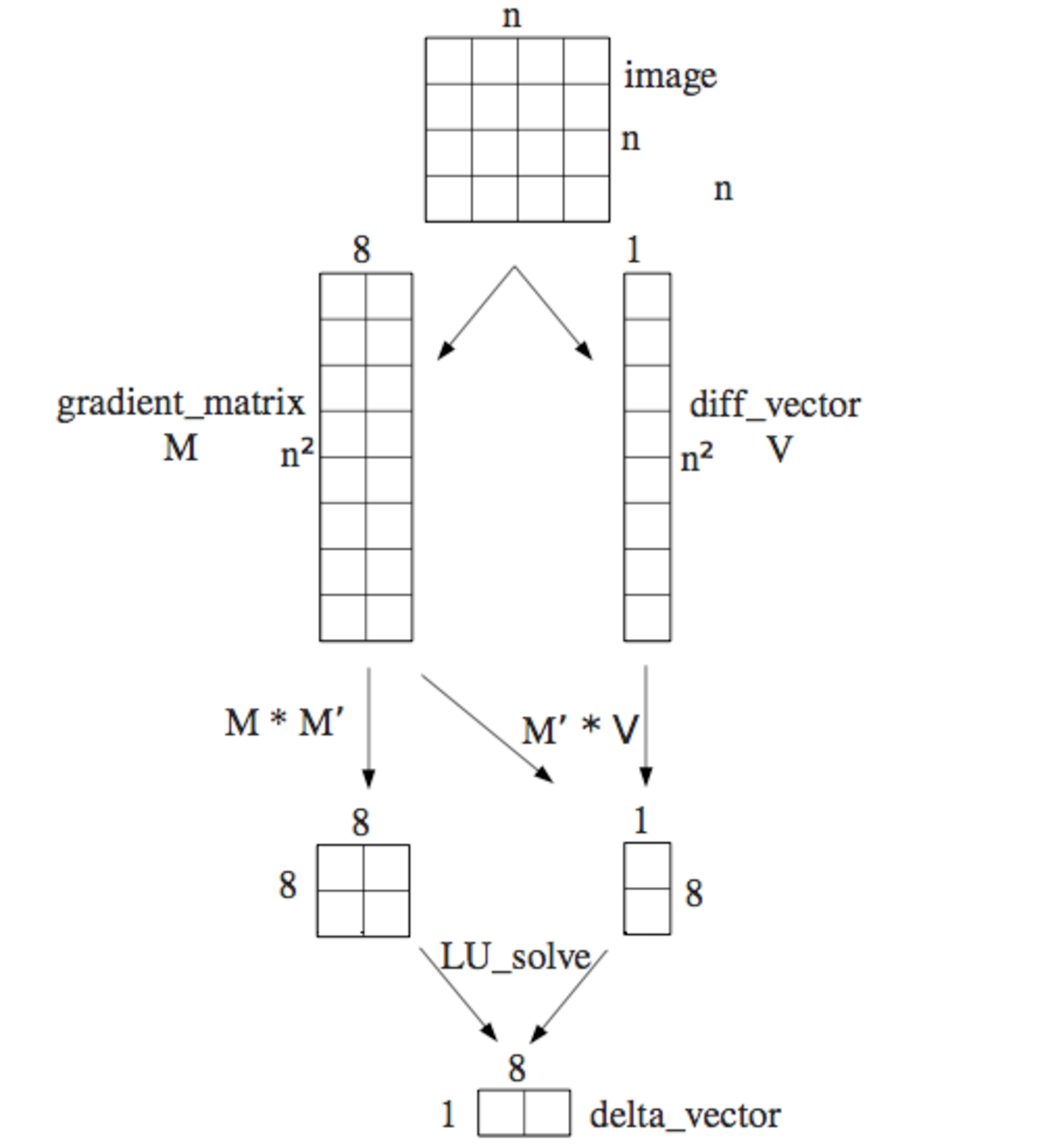
\includegraphics[width=115mm,height=130mm]{./algorithm}%
\label{steps}}
\caption{Gauss-Newton algorithm steps}
\end{figure}
\subsection{Parallel Schemes}

As a first thing we have to model the parallel computation using a structured parallel programming scheme. We know that there is an (ideal) infinite stream of images and the computation is a pure function, hence a way to parallelize this program can be the farm approach: we can replicate the algorithm in each worker following the cost model that we will introduce soon. For this scheme is not necessary to know the internal structure of the algorithm, but if we analyse it, we recognize some interesting aspects.

Following the pseudo code in Figure 1 we have:
\begin{enumerate}
\item the construction of the \textit{diff\_vector} and the \textit{gradient\_matrix} starting from the image.
\item the multiplication between the \textit{gradient\_matrix} and its own transposed matrix, that is the main operation.
\item the multiplication between the transposed matrix and the \textit{diff\_vector}.
\item the LU\_solve operation
\item the sum of the vector \textit{parameter} with \textit{delta\_vector}.
\end{enumerate}

From above, we can notice that the first three points could be executed in local in a module if we know a partition of the \textit{gradient\_matrix} and a partition of the \textit{diff\_vector}. In particular, if we consider very fine grain computations, we notice that it is sufficient to have a single element of the matrix and a single element of the vector for computing the partial multiplications between elements. This means that there is no need of communications of values between different partitions of the matrix but it is necessary to communicate the partial results in such way it is possible to sum them and to obtain the $8$x$8\ gradient\_matrix$ and the vector $gradient\_vector$. Finally, we notice that the fourth and the last point must be executed only after the calculations above and they take a negligible time respect than the previous operations.

This situation suggests a parallelism scheme in which the data can be partitioned between different modules for computing the first three points and after we need a reduce communication for obtain the final results and execute the last two parts of the algorithm. This means that our program can be parallelized through a map reduce too.

At this point we chose to realize both a farm and data parallel scheme. We will further discuss their cost model in the next section.
\section{Cost Model}

In this section we will talk about the cost models of the farm and data parallel paradigms used to parallelize the algorithm above. In both of them there is replication of the function in every worker, but in the second we have partition of data. The methodology used for measure the performance is based on standard measures, in particular we have taken principally into account the service time and the scalability. These cost models are based on another cost model regarding the communications between processes: the latency of a send is composed by a fixed term $T_{setup}$ independent from the message length, and by a term $T_{trasm}$ variable in the length of the message.

When we instantiated the problem, we assumed that the emitter in the farm and the scattering module in the data parallel have always an image ready to send. In this way we simulated the minimal interarrival time of images from another module generating the stream (that it will be the camera module during the real behaviour of this application).

\subsection{Farm}

The most important parameter of this paradigm, that is working with computations based on stream, is the service time $T_{s}$. In the farm, the emitter, the generic worker and the collector are organized in pipeline, hence it is equal to
\[
T_{s} = \max \lbrace T_{e}, T_{w}, T_{c}\rbrace
\]
where, in this specific case, the service time of the emitter (called $T_{e}$) is equal to the communication latency $L_{image}$ for sending an image and the collector service time $T_{c}$ is negligible respect $T_{e}$ because this module sends only the result of the computation. Following the considerations above the term $L_{image}$ is equal to minimum interarrival time $T_{a}$ at the system. According to queuing theory we have that the service time $T_{s}$ of the farm system is equal to the interarrival time $L_{image}$ if
\[
T_{w} = L_{image} \Leftrightarrow \frac{T_{image}}{nw} = L_{image} \Leftrightarrow nw = \frac{T_{image}}{L_{image}} 
\]
where $T_{image}$ is the time spent to execute the Gauss-Newton algorithm over an image and $nw$ is the ideal number of workers. If the purpose is to maximize the bandwidth (loosing a few in efficiency) we can choose the ceiling of this value.

If we let $m$ as the stream length, the completion time can be evaluated as
\[
T_{C} = nw \cdot L_{image} + \frac{m}{nw} \cdot T_{w} + T_{c} 
\]
where $\frac{m}{nw}$ is the mean number of tasks for worker.
If we have that $m \gg nw+2$ (stream length is more bigger than the number of modules of the farm), like in this project, we can consider the completion time close to
\begin{equation}
\label{completiontime}
T_{C} \simeq m \cdot T_{s}
\end{equation}
The scalability is a measure of how much speed is the computation respect than the sequential case. Formally, it is defined as
\begin{equation}
\label{scalability}
s = \frac{T_{image}}{T_{s}}
\end{equation}
where $T_{s}$ changes in function of the parallelism degree $n=nw+2$.

The Gauss-Newton algorithm practically executes a function for each pixel in the image. The time spent for this function is not variable considering different pixel values, hence we have the maximum loading balance and a round-robin strategy is a well solution. But if this condition was not valid, it was important to find a scheduling solution for balancing the load like, for instance, an on-demand strategy. As we will see in the next sections, the tests will confirm that there is not difference about the circular assignment of images and the on-demand strategy in this project.

\subsection{Map Reduce}

The data parallel paradigm can be able to reduce the latency of the computation, but in this case it operates on a stream of elements hence the most important parameter is yet the service time. As we said, the data parallel computation used for this parallel program is a map with reduce. In this case each worker computes the algorithm on own partition of data, hence there is not need to have communications between workers but it is necessary to have scatter and reduce communications. The scheme of these communications is very important: in the simplest case we have $nw$ send from or to the workers but is possible to think about tree schemes where the latency becomes logarithmic in the number of workers and no more linear. Another aspect to take into account is how to partition the pixels of the image: it can be done by rows, columns or in an interleaving way. In particular, we decided to partition the elements of the $gradient\_matrix$ and the $diff\_vector$ by rows obtaining a minimum number of cache faults. However, in this section we are not interesting in details regarding the implementation but our cost model will take in consideration these choices.

In the most general case for a map reduce operating on a stream of elements, the service time can be evaluated as
\[
T_{s} = \max\lbrace T_{scatter}, T_{w}, T_{reduce}\rbrace
\]
because, like in the farm, we have a pipeline behaviour. Obviously, $T_{w}$ is the time spent for execute our algorithm over a partition of the image. We obtain that the map is not bottleneck if we choose $nw$ workers such that
\[
nw = \frac{T_{image}}{L_{image}}
\]
and considering scatter and reduce realized in an opportune scheme such that
\[
T_{scatter} \leq L_{image}
\]
\[
T_{reduce} \leq L_{image}
\] 
In this specific case the associative function of the reduce is simply a sum over the partial results obtained by the execution of the algorithm over the single partitions of the image. This means, as we said in Section 1.3, that the time spent for this operation is negligible respect than the functions in the workers hence there is not need to realize it using a tree but it is sufficient to use only a module. This module will be able to execute the the last two functions described in the Section 1.3 too. In this project, the considerations about the linear or logarithmic latency are principally referred to the scatter.

The completion time is evaluated like in Formula \ref{completiontime} and the scalability is the same of Formula \ref{scalability}.

\subsection{Farm vs Map}

In general the data parallel solutions require less memory capacity of the architecture nodes respect than the farm scheme. If we think that in the ideal case the entirely data structures of the program should be present in main memory, to have only a single computation over an image respect than different computations over different images can be an advantage from the point of view of the swap information. This can become important in shared memory architecture especially when we increase the grain of the data input.

This latter aspect is fundamental too: to have an optimal dimension of the input data permits to increase the benefits because, in according to our communications cost model above, we can amortize the $T_{setup}$ cost. In the data parallel form this means to found the dimension of the partitions (hence the parallelism degree) of the matrix, instead in the farm this means to have an adequate dimension of the input images. We tested our parallel program in both the paradigms with different data grain in such a way to recognize the situations above.

From above we know that in both the solutions the number of workers $nw$ is the same, hence the parallelism degree of our application becomes
\begin{itemize}
\item $nw+2$ in the farm
\item $nw+n_{scatter}+1$ in the map reduce
\end{itemize}
If the linear scatter is not a bottleneck we have the same parallelism degree of the farm, otherwise some nodes of our architecture will be allocate with service processes. This means an decrease of the performance principally in architecture with a low number of nodes. For verify this, our data parallel will be able to use a single node for the communications instead of the classic behaviour. We will see these things in the next sections.
\section{Implementation}
\section{Test}

Test were performed on bla bla bla
process services are bla bla
communication on MPI?
hostfile on axth

\begin{figure}[p]
\centering
\subfigure[]{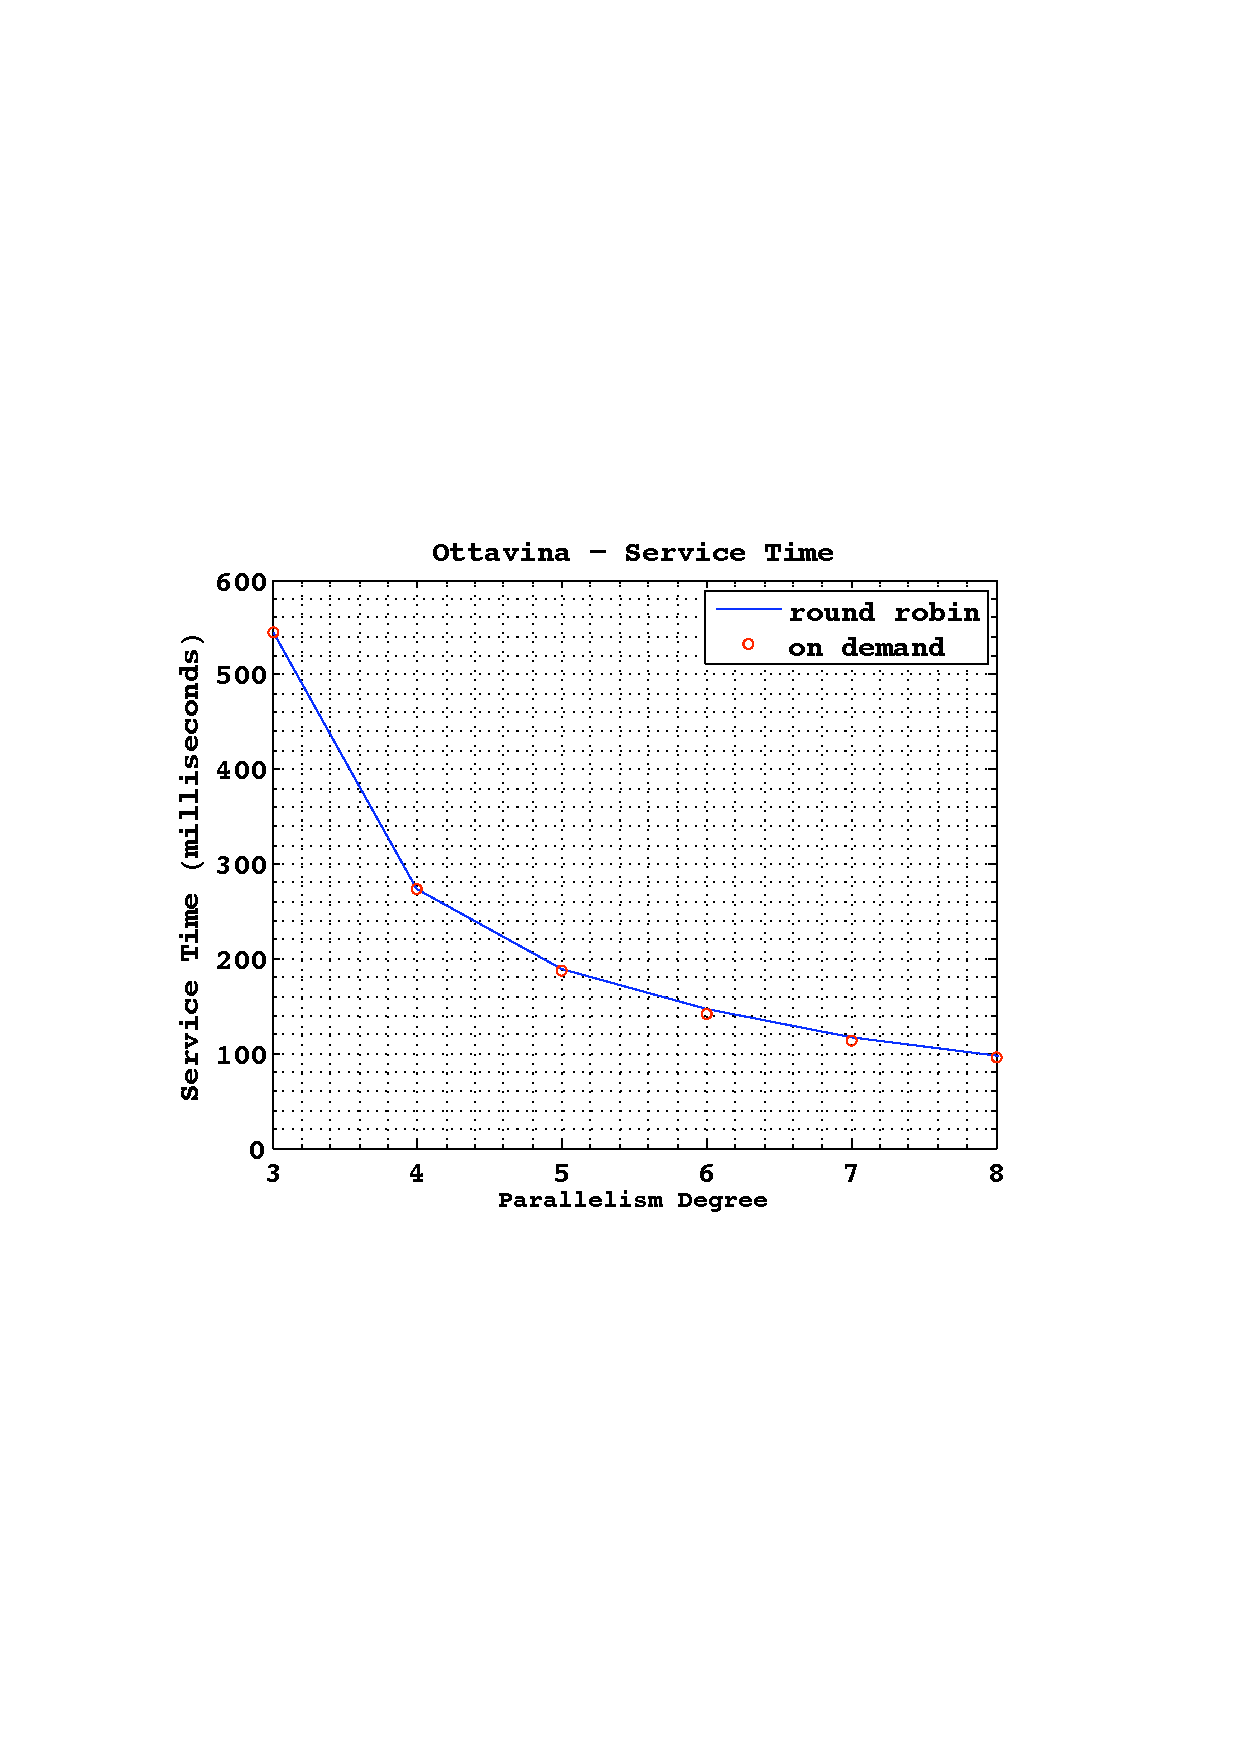
\includegraphics[width=\columnwidth,height=3.5in]{./CHART/ottavina_farm_1000_time}%
\label{graf:ottavina_farm_1000_time}}
\subfigure[]{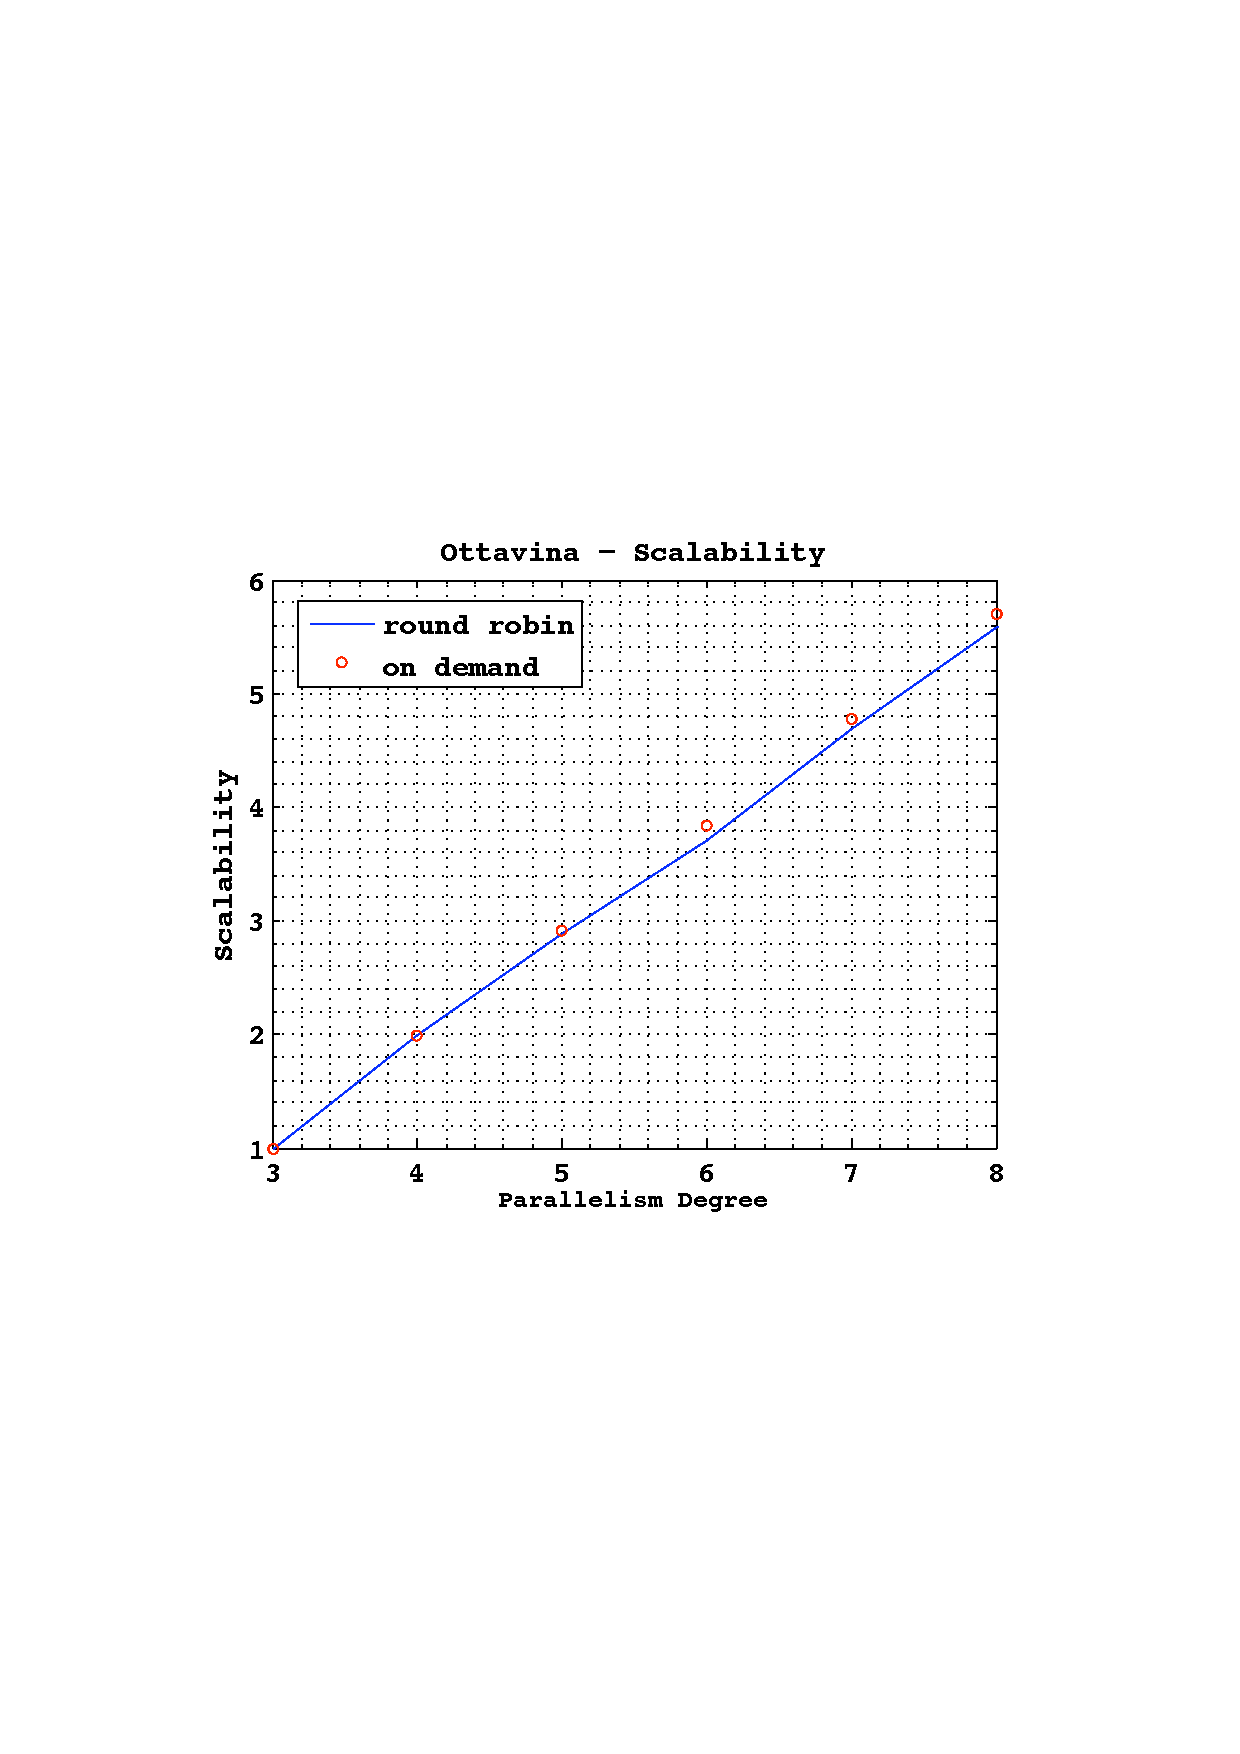
\includegraphics[width=\columnwidth,height=3.5in]{./CHART/ottavina_farm_1000_scala}%
\label{graf:ottavina_farm_1000_scala}}
\caption{ Service time of the farm implementation \ref{graf:ottavina_farm_1000_time} and relative scalability \ref{graf:ottavina_farm_1000_scala}. Test performed on Intel E5420 @ 2.50 Ghz cpu with images of $10^6$ 8bit pixels. Parallelism degree is starting from 3 because of the service nodes (emitter and collector). }
\label{chart:ottavina_farm_1000}
\end{figure}

\begin{figure}[p]
\centering
\subfigure[]{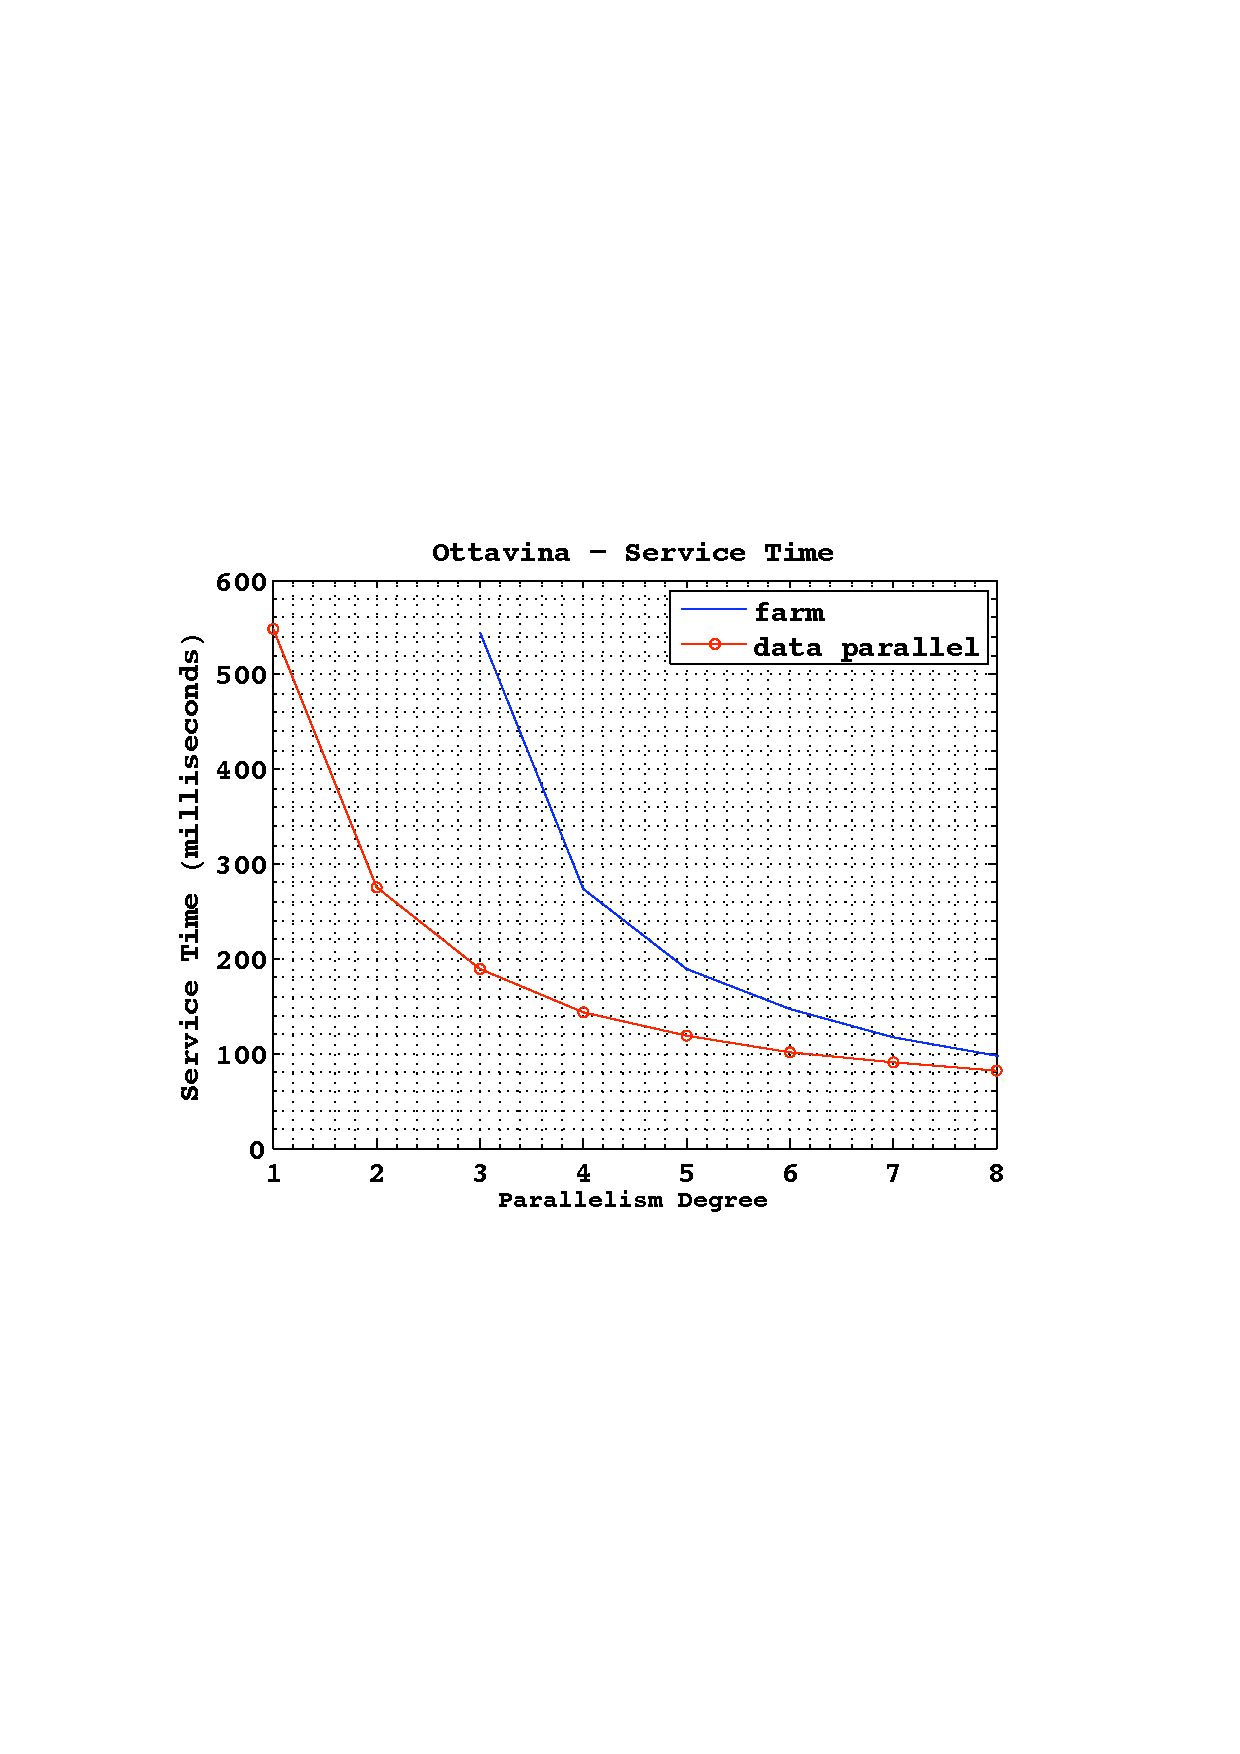
\includegraphics[width=\columnwidth,height=3.5in]{./CHART/ottavina_farmvsdata_1000_time}%
\label{graf:ottavina_data_1000_time}}
\subfigure[]{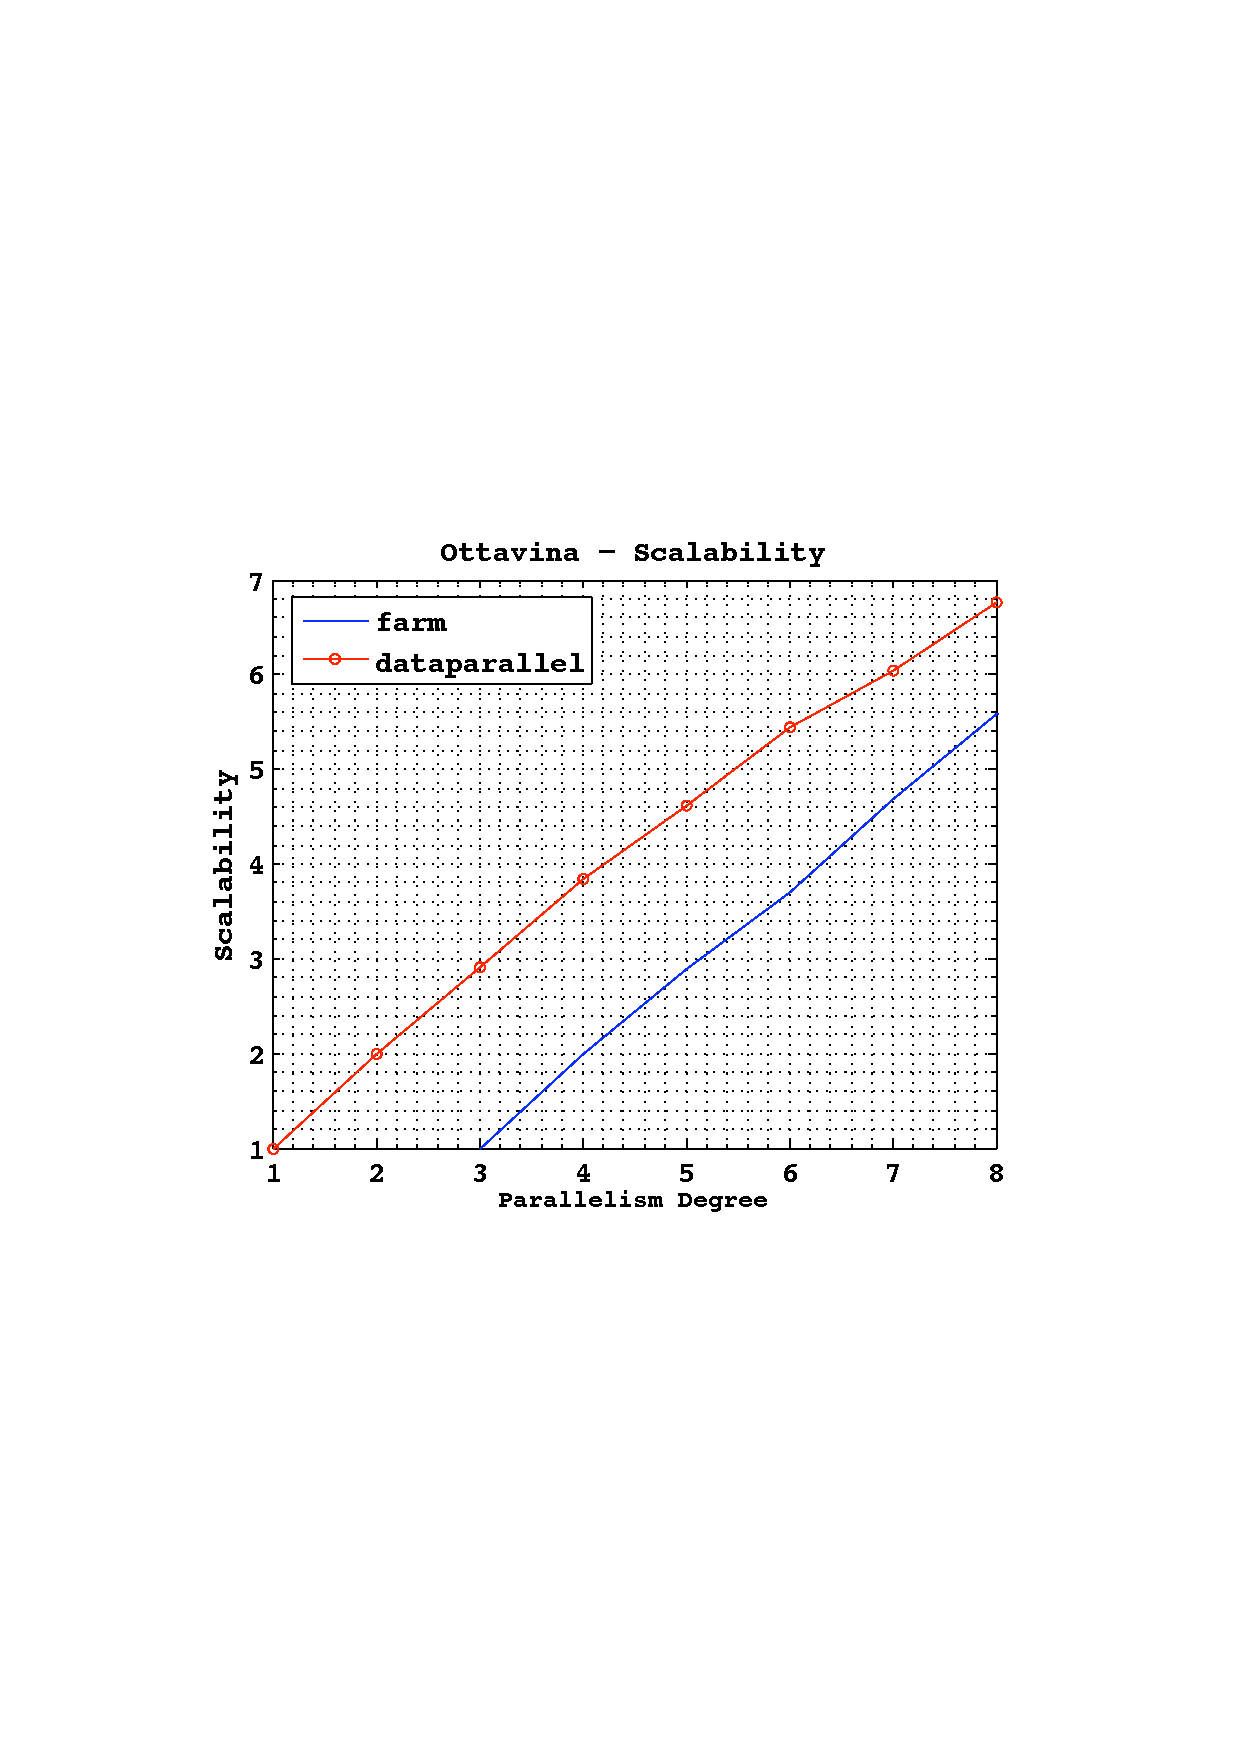
\includegraphics[width=\columnwidth,height=3.5in]{./CHART/ottavina_farmvsdata_1000_scala}%
\label{graf:ottavina_data_1000_scala}}
\caption{ Service time of the farm and data parallel implementation \ref{graf:ottavina_farm_1000_time} and relative scalabilities \ref{graf:ottavina_farm_1000_scala}. Test performed on Intel E5420 @ 2.50 Ghz cpu with images of $10^6$ 8bit pixels.}
\label{chart:ottavina_data_1000}
\end{figure}

\begin{figure}[p]
\centering
\subfigure[]{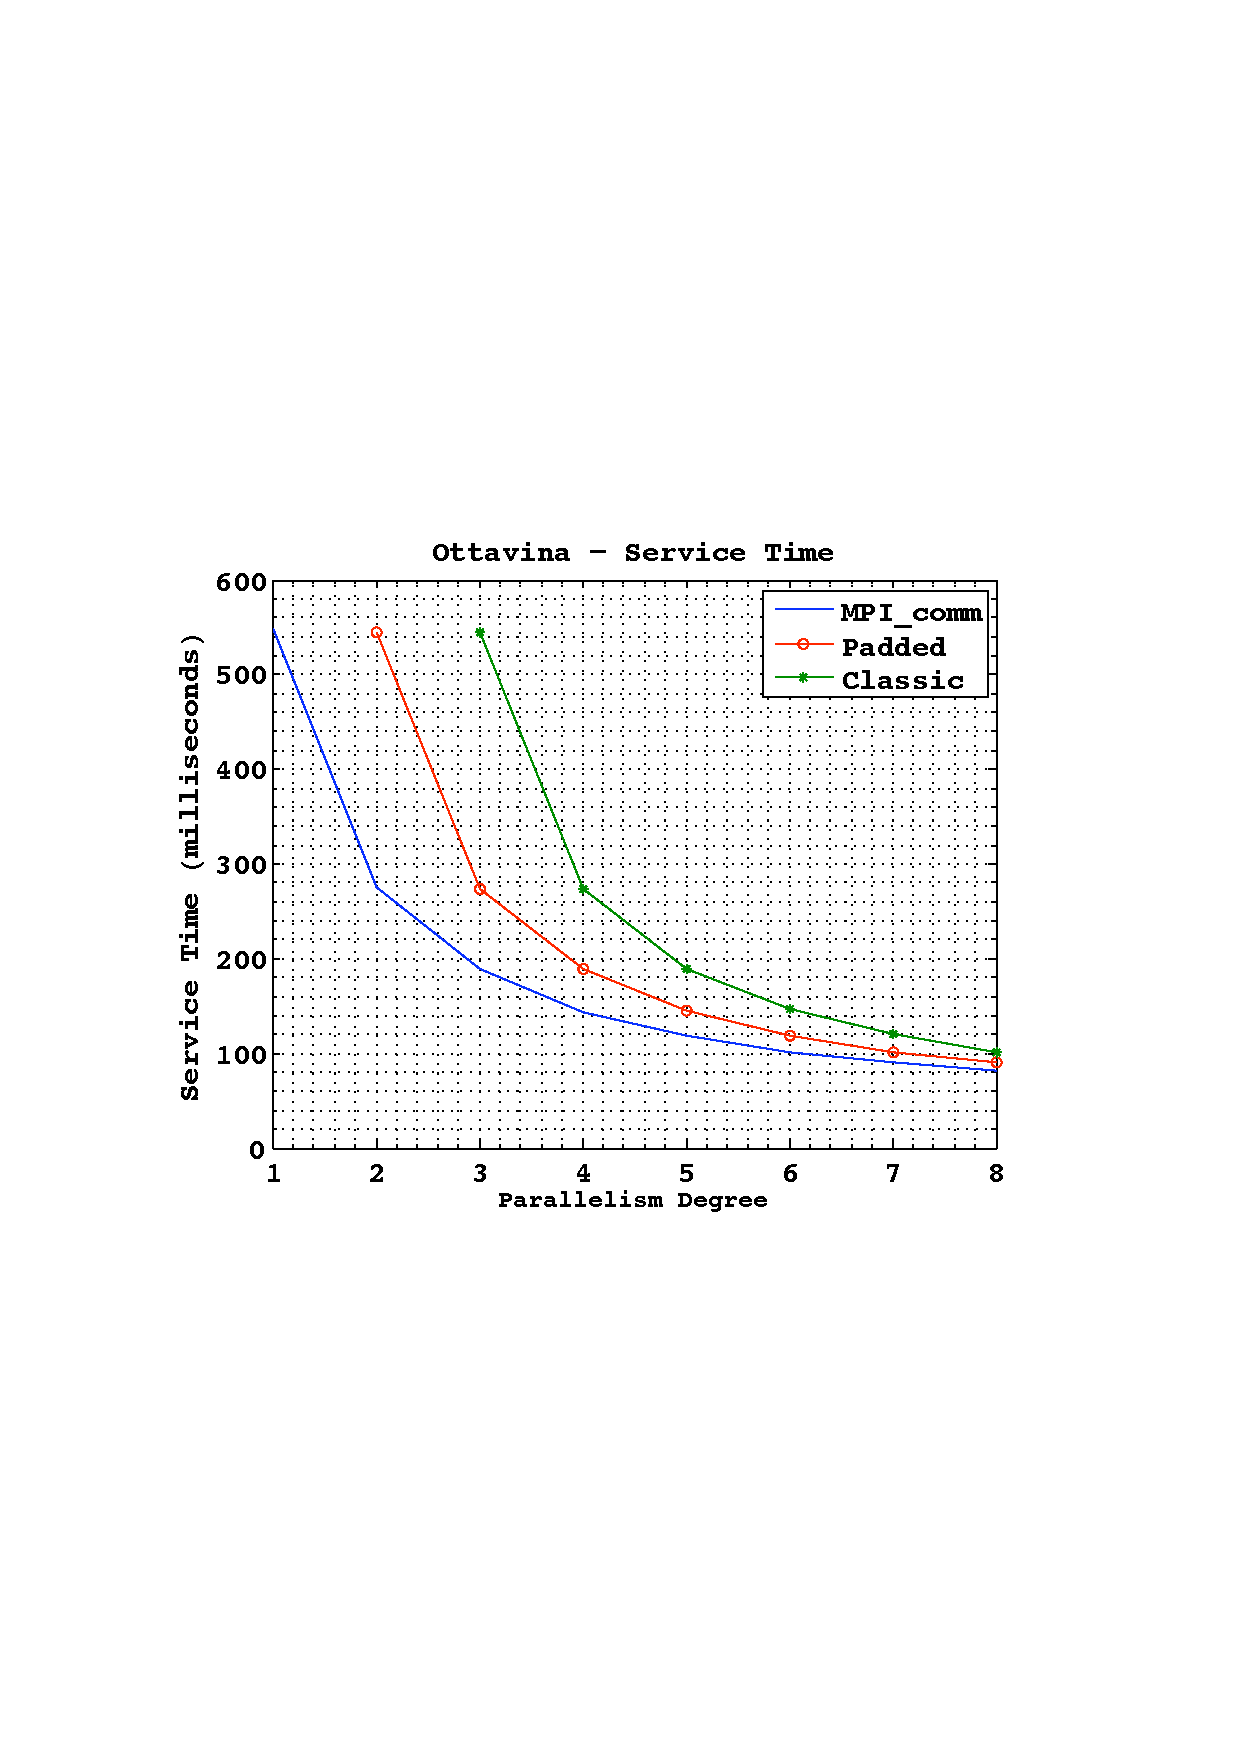
\includegraphics[width=\columnwidth,height=3.5in]{./CHART/ottavina_alldata_1000_time}%
\label{graf:ottavina_alldata_1000_time}}
\subfigure[]{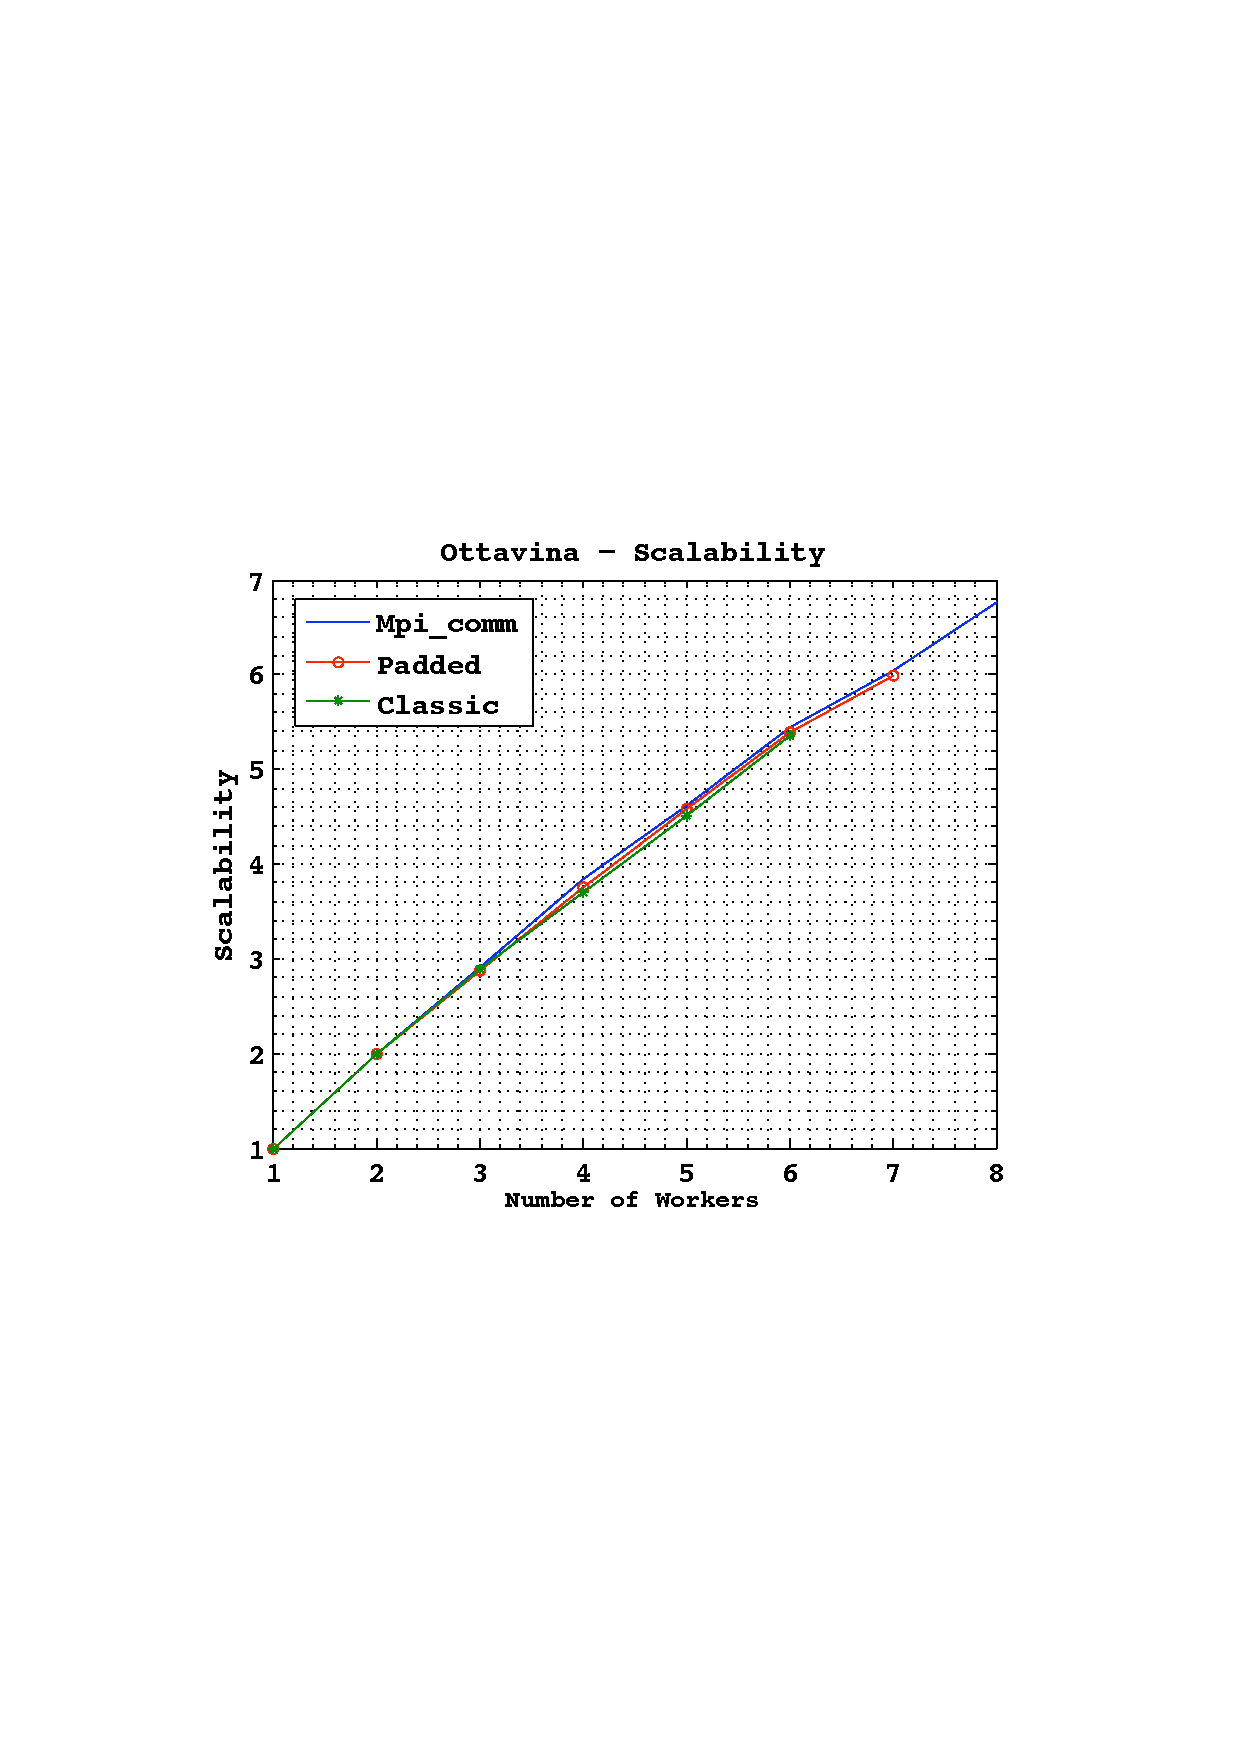
\includegraphics[width=\columnwidth,height=3.5in]{./CHART/ottavina_alldata_1000_scala}%
\label{graf:ottavina_alldata_1000_scala}}
\caption{ Service time of all the data parallel implementation \ref{graf:ottavina_farm_1000_time} and relative scalabilities, normalized with respect of the number of workers \ref{graf:ottavina_farm_1000_scala}. Test performed on Intel E5420 @ 2.50 Ghz cpu with images of $10^6$ 8bit pixels.}
\label{chart:ottavina_alldata_1000}
\end{figure}

\begin{figure}[p]
\centering
\subfigure[]{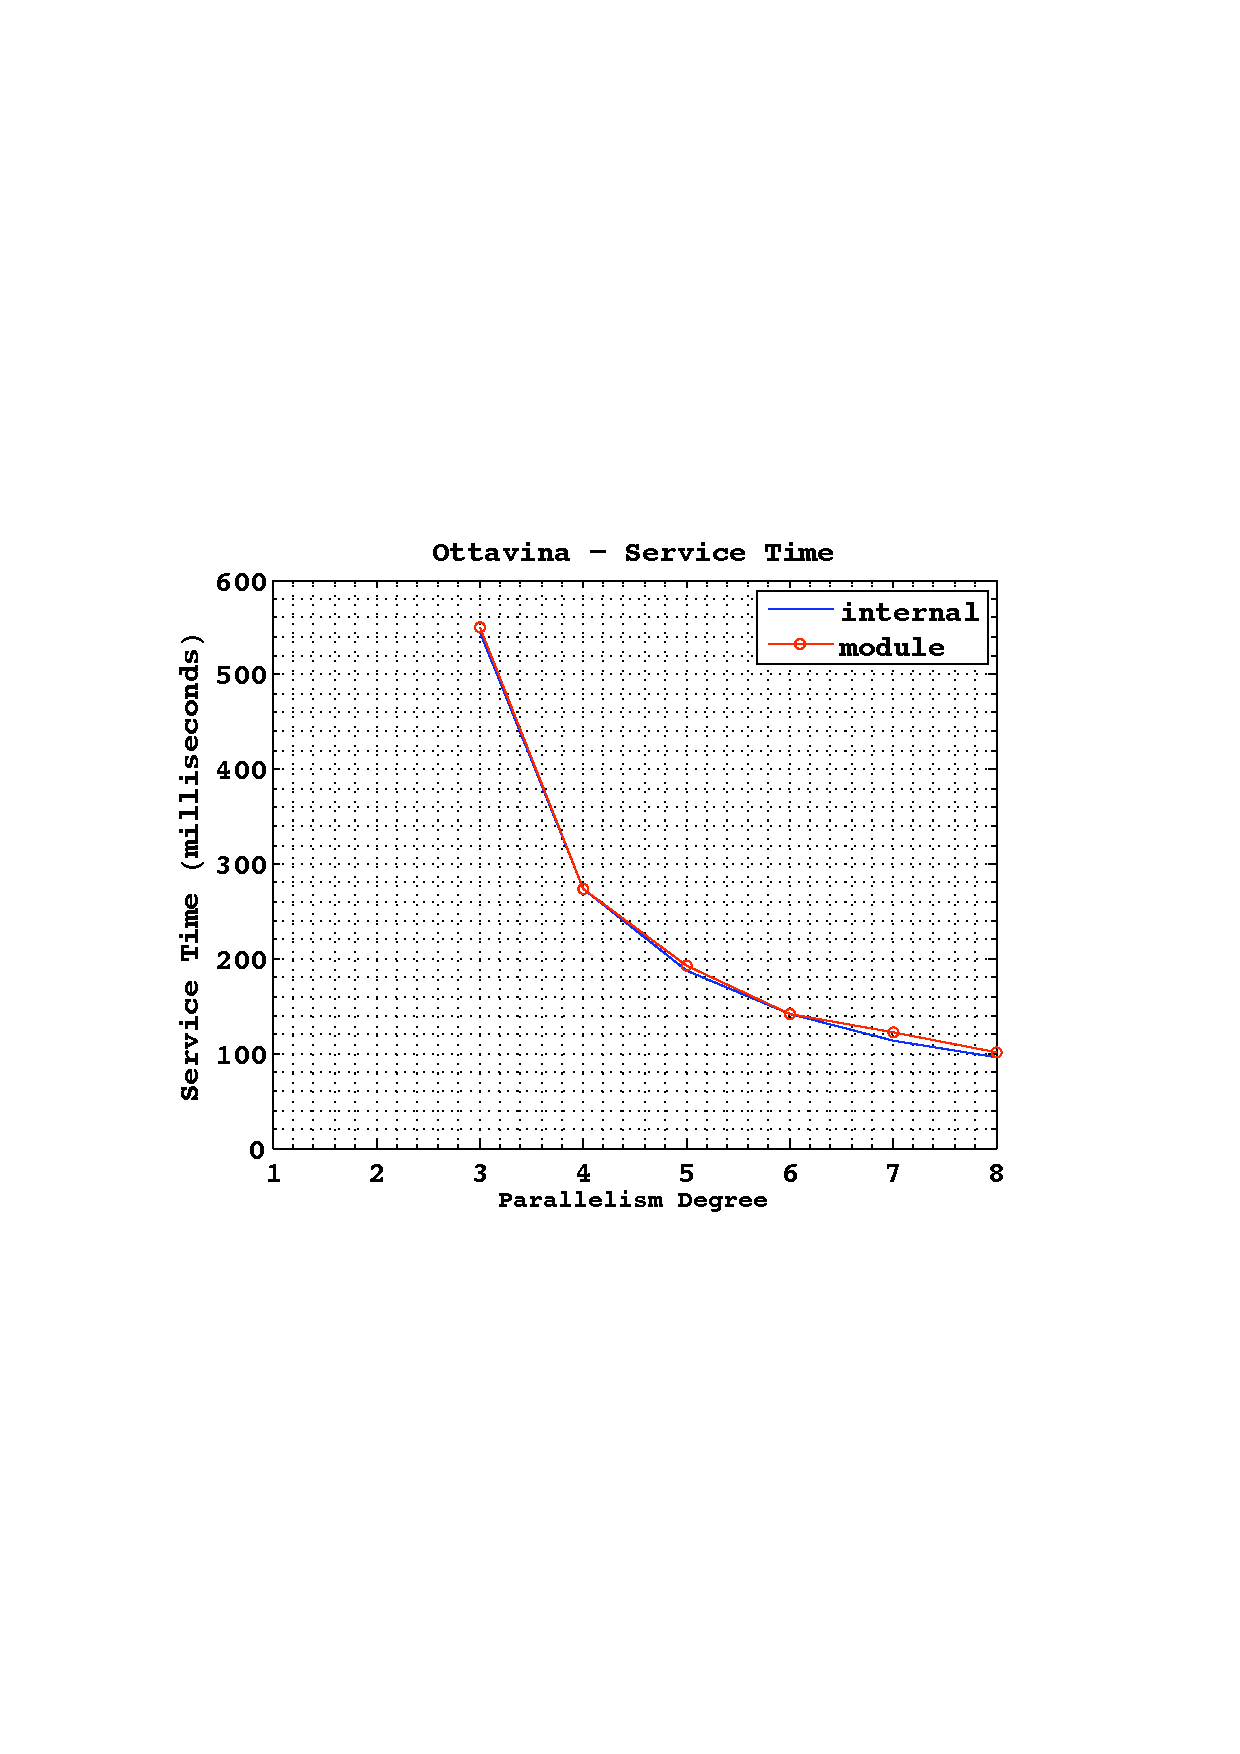
\includegraphics[width=\columnwidth,height=3.5in]{./CHART/farm_camera}%
\label{graf:farm_camera}}
\subfigure[]{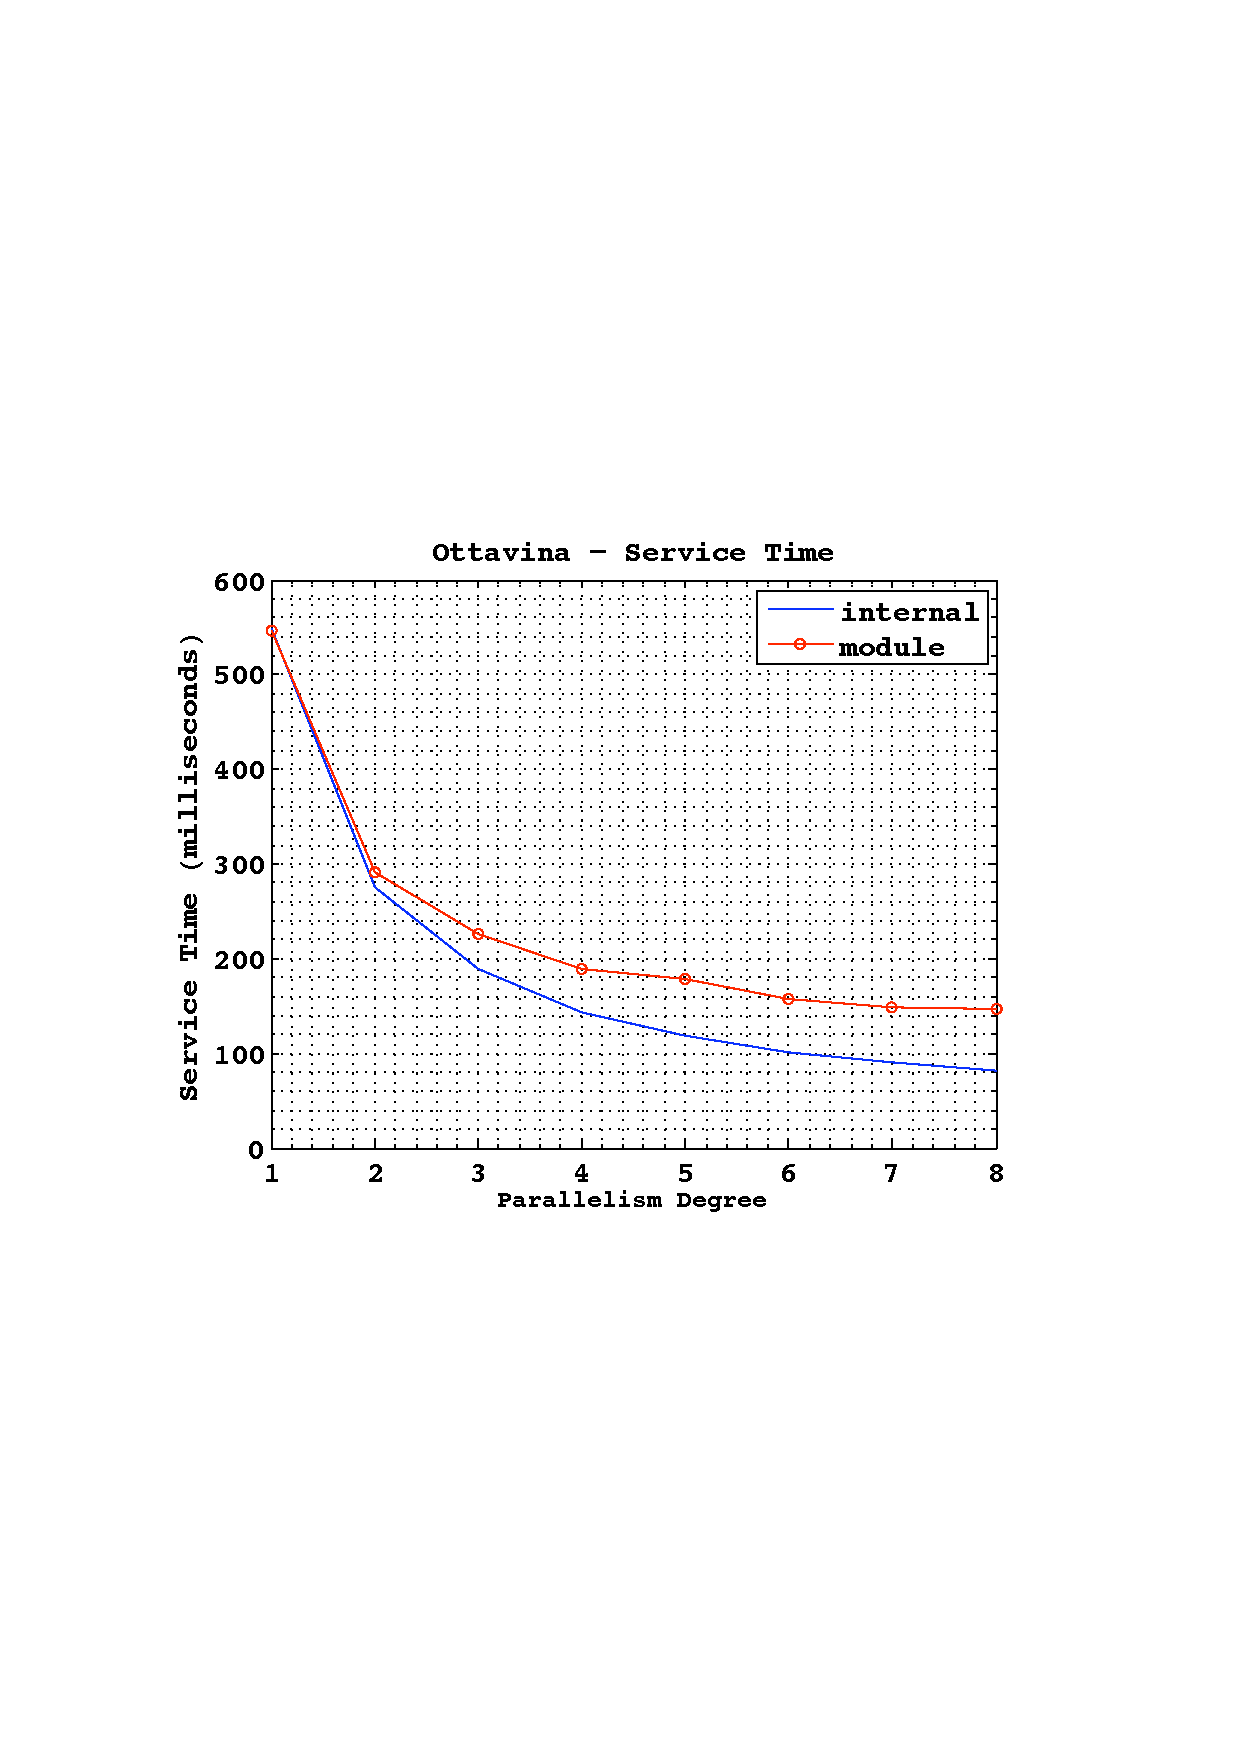
\includegraphics[width=\columnwidth,height=3.5in]{./CHART/data_camera}%
\label{graf:data_camera}}
\caption{ Comperison of application service time of farm implementation \ref{graf:ottavina_farm_1000_time} and data parallel implementation  \ref{graf:ottavina_farm_1000_scala} with or without external camera module. Test performed on Intel E5420 @ 2.50 Ghz cpu with images of $10^6$ 8bit pixels.}
\label{chart:ottavina_camera}
\end{figure}

\begin{figure}[p]
\centering
\subfigure[]{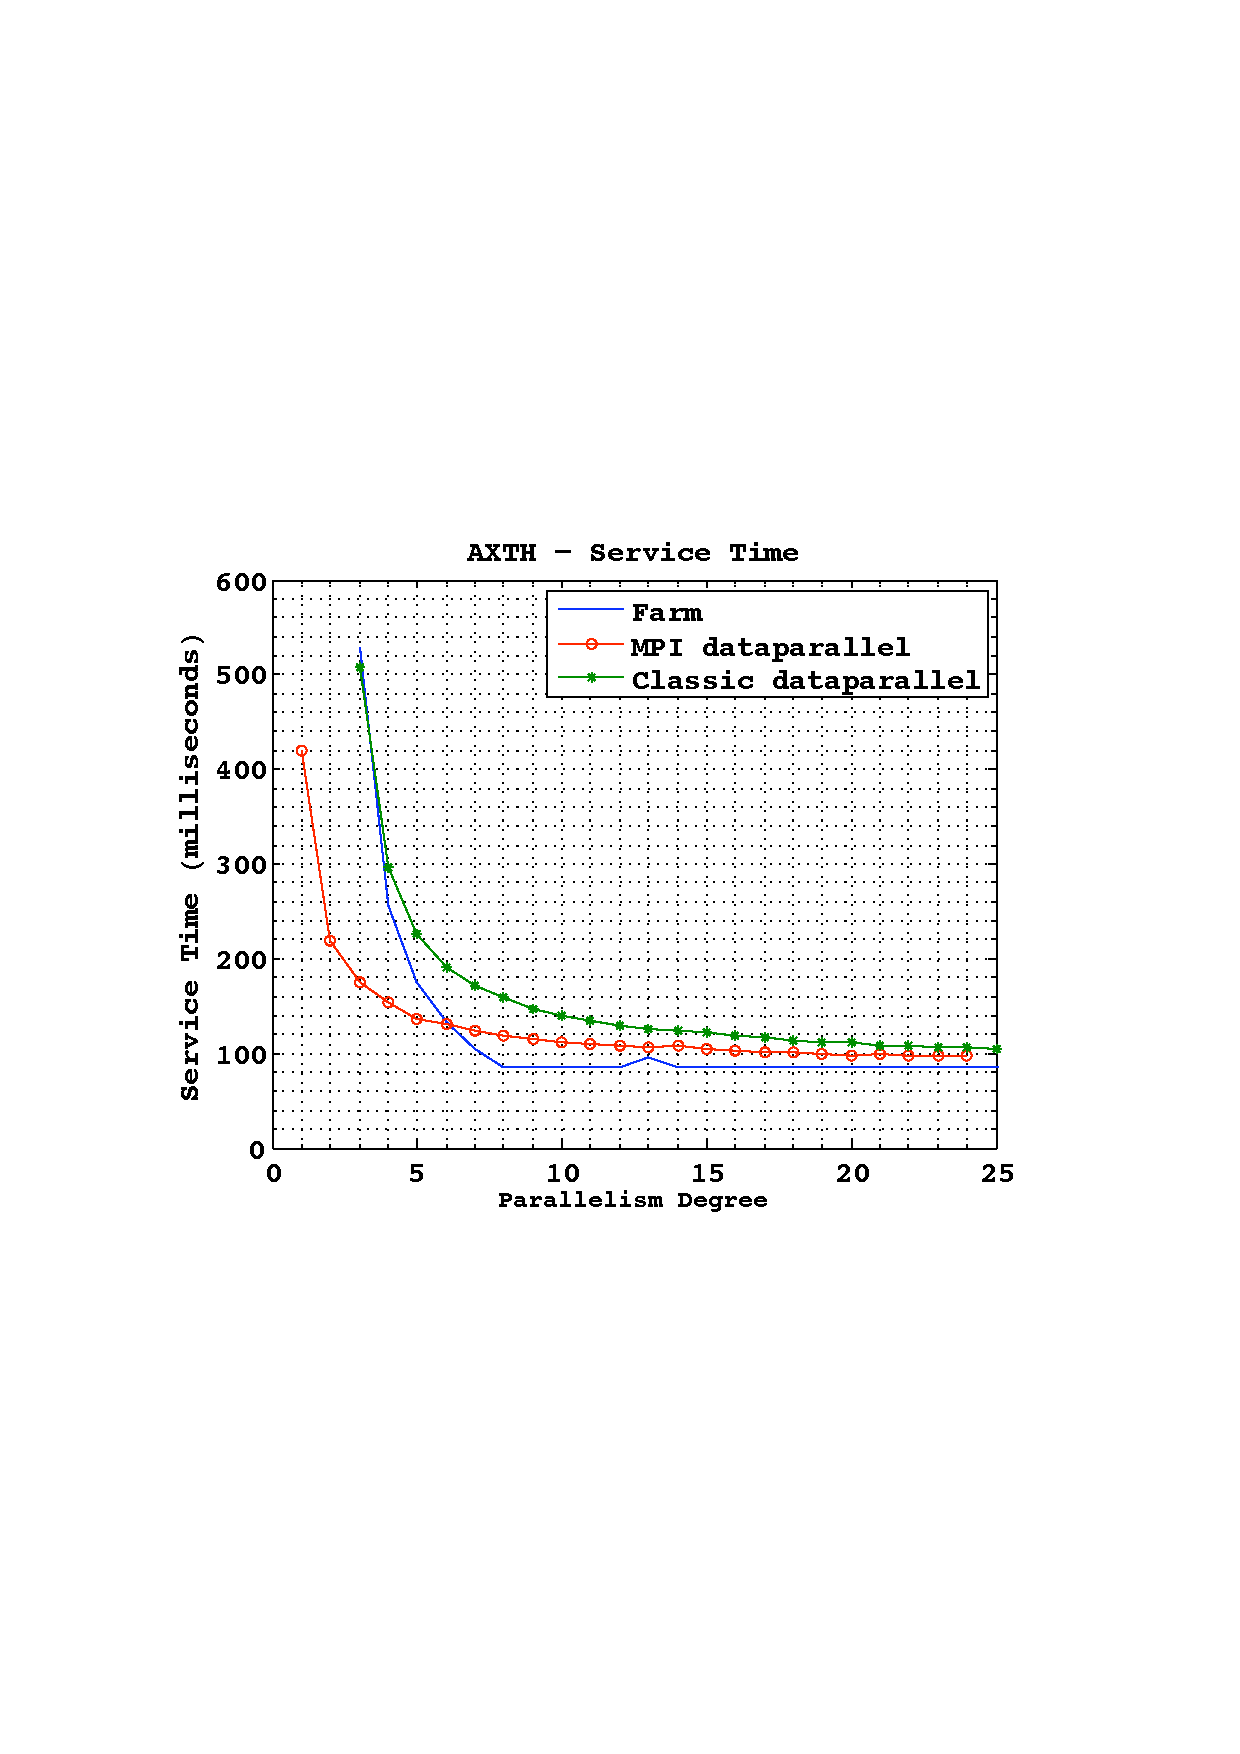
\includegraphics[width=\columnwidth,height=3.5in]{./CHART/axth_confronto_time}%
\label{graf:time_axth}}
\subfigure[]{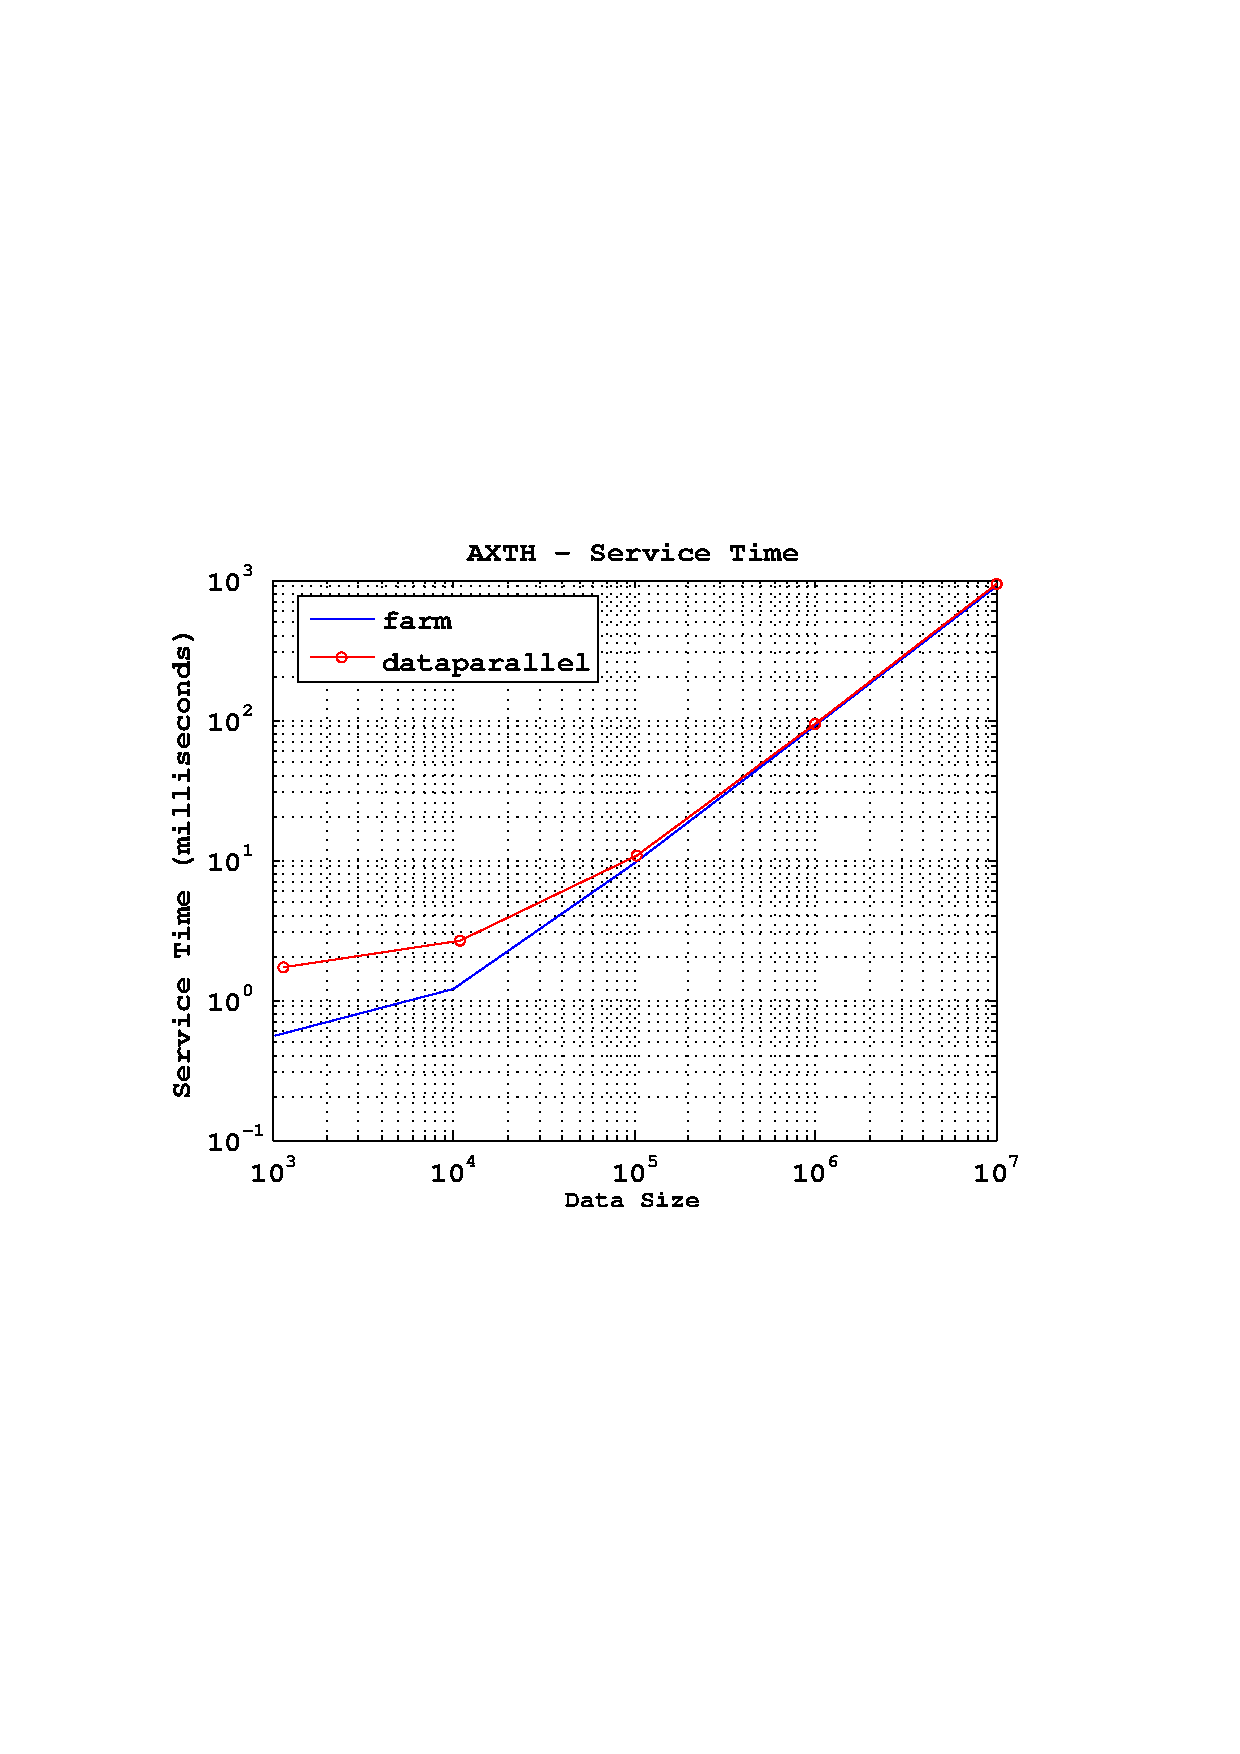
\includegraphics[width=\columnwidth,height=3.5in]{./CHART/axth_scalability}%
\label{graf:scala_axth}}
\caption{ Comparison of application service time of the various implementation \ref{graf:time_axth} and relative Scalability \ref{graf:scala_axth}. Test performed on a set of 20 nodes with Intel E7400 @ 2.80 Ghz cpu. Images of $10^6$ 8bit pixels.}
\label{chart:axt}
\end{figure}

\begin{figure}[p]
\centering
\subfigure[]{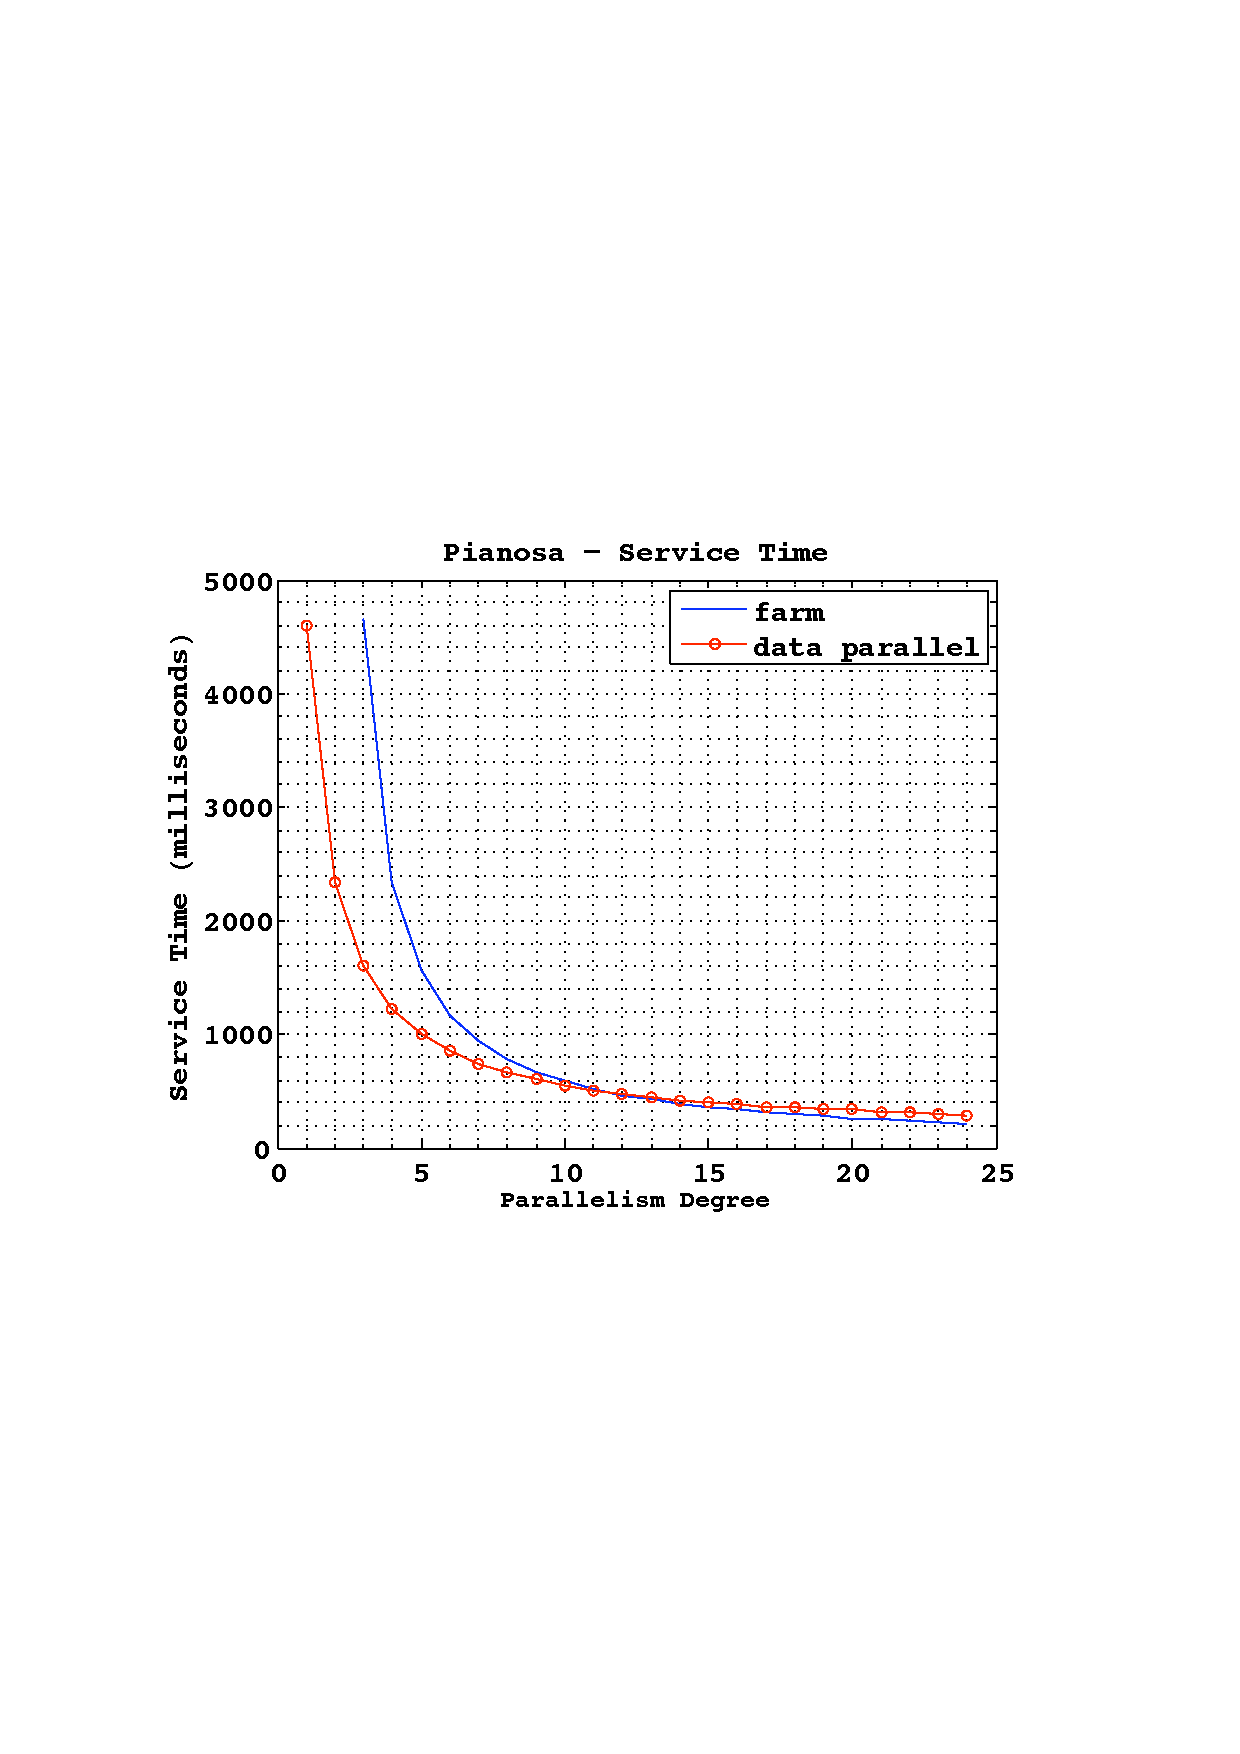
\includegraphics[width=\columnwidth,height=3.5in]{./CHART/pianosa_time3}%
\label{graf:pianosa_time}}
\subfigure[]{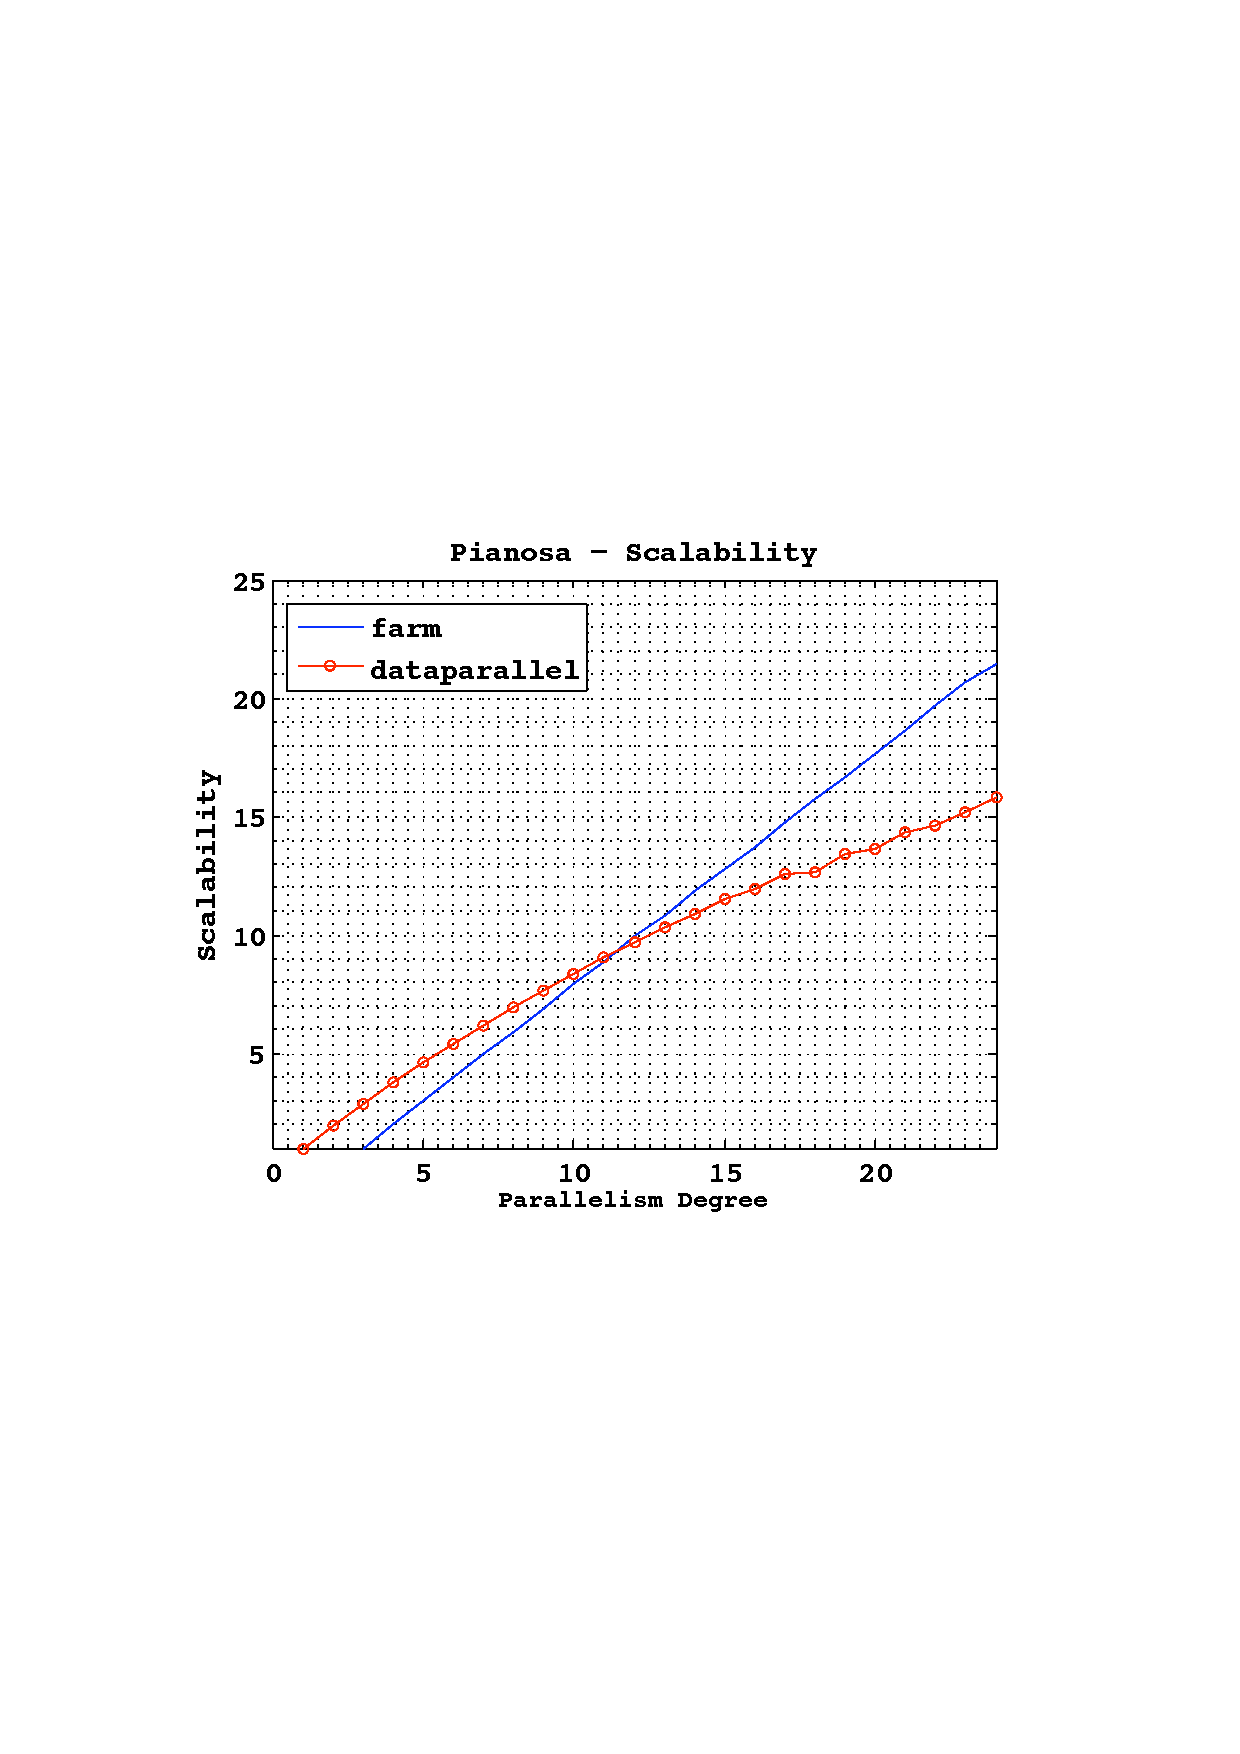
\includegraphics[width=\columnwidth,height=3.5in]{./CHART/pianosa_scala}%
\label{graf:pianosa_scala}}
\caption{ Service time on the Pianosa cluster of farm and data parallel implementation \ref{graf:time_axth} and relative scalability \ref{graf:pianosa_scala}.  Test is performed on a set of 24 nodes with Intel Pentium III @ 800 Mhz cpu. Images of $10^6$ 8bit pixels.}
\label{chart:pianosa_comm}
\end{figure}

\begin{figure}[p]
\centering
\subfigure[]{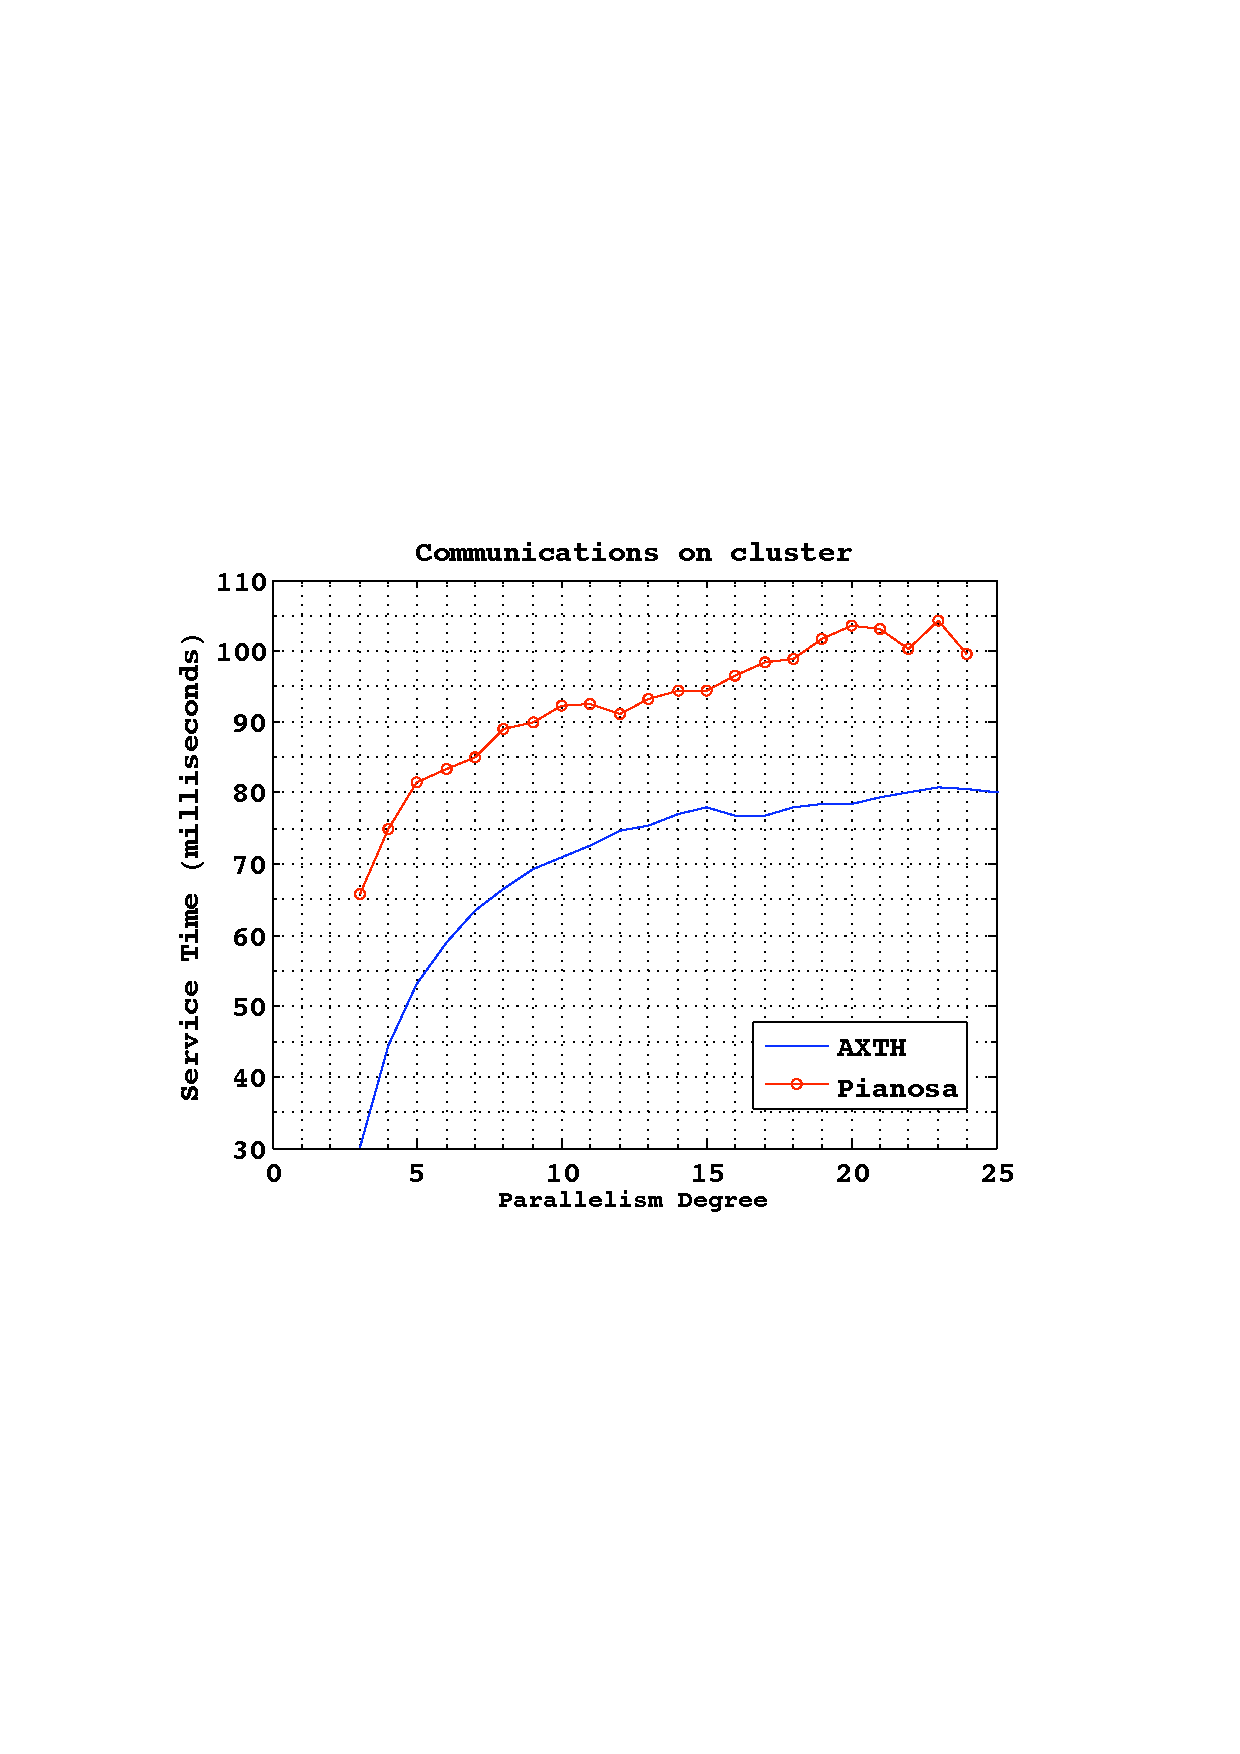
\includegraphics[width=\columnwidth,height=3.5in]{./CHART/Communication}%
\label{graf:communication}}
\subfigure[]{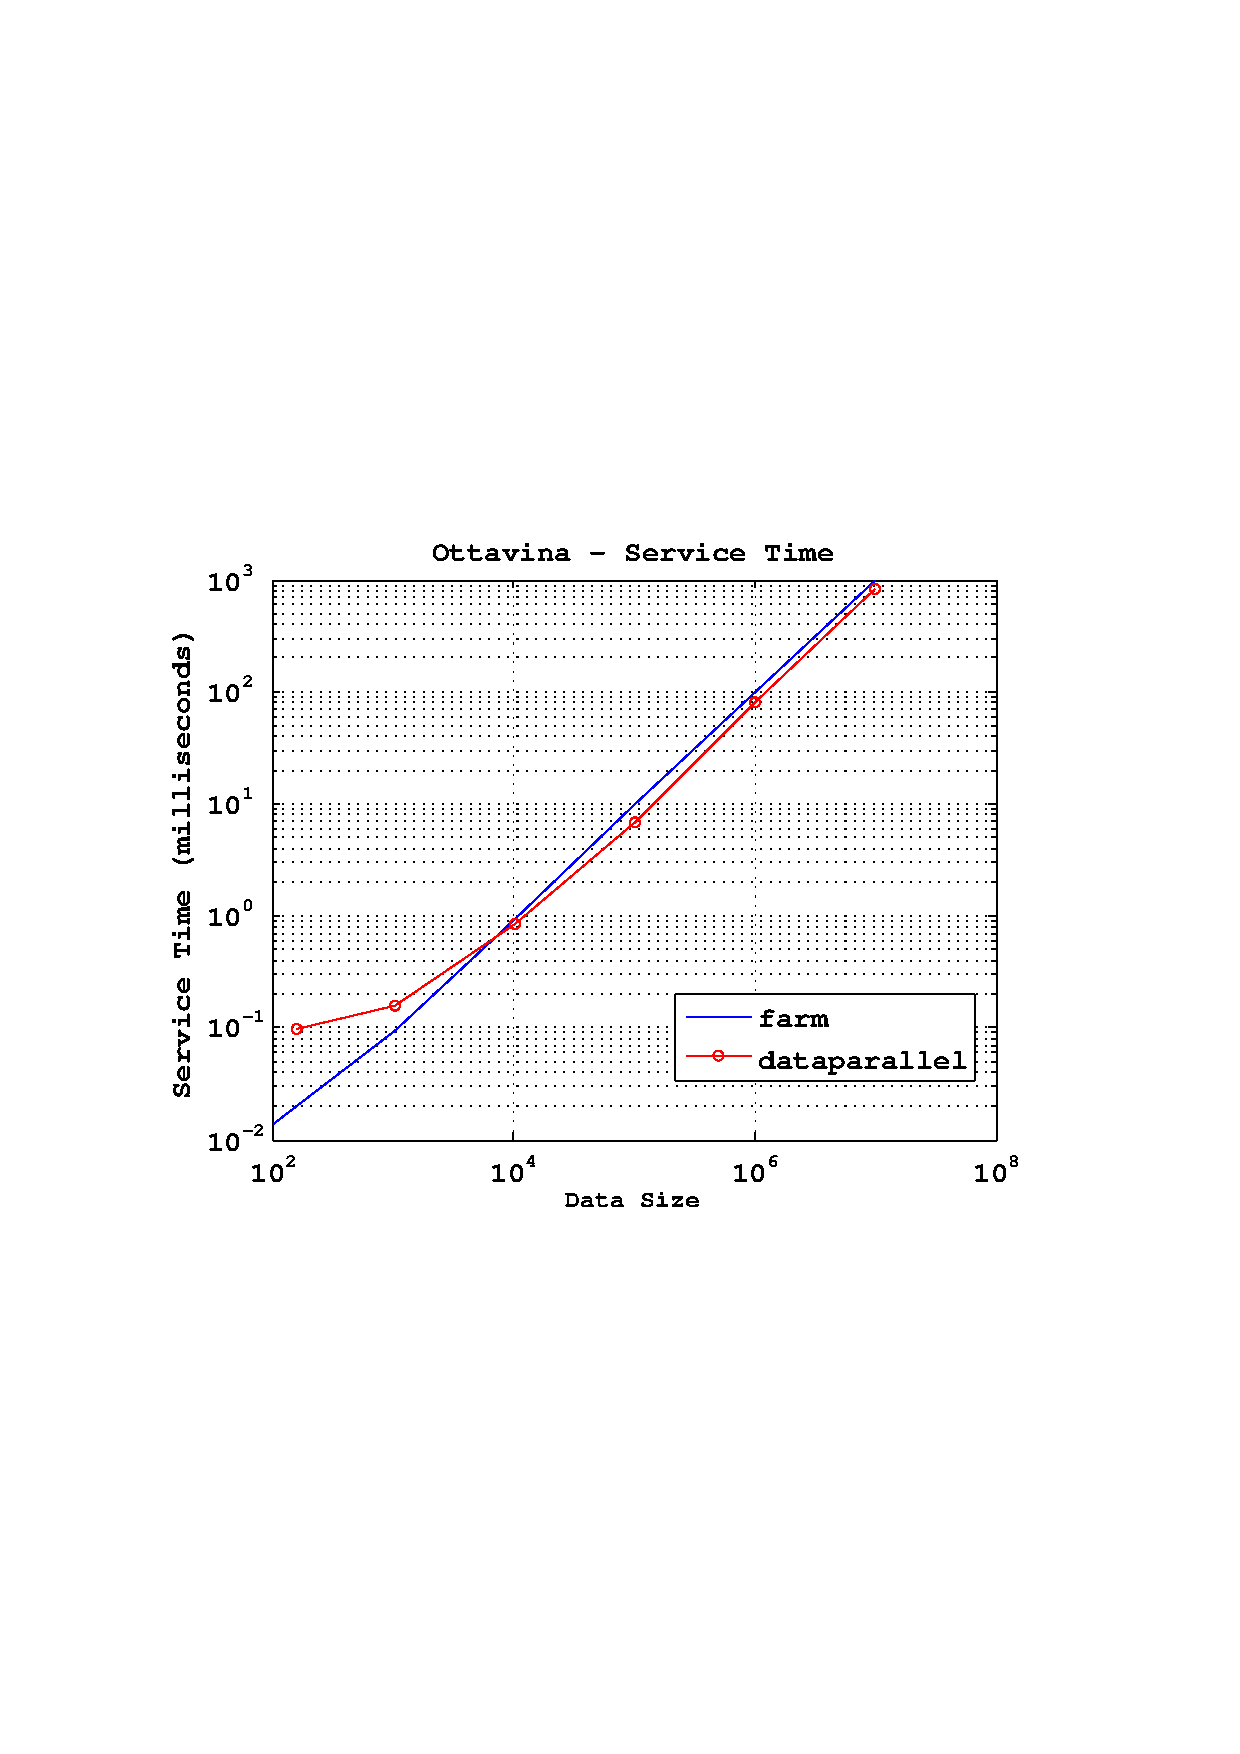
\includegraphics[width=\columnwidth,height=3.5in]{./CHART/ottavina_datascale}%
\label{graf:ottavina_datascale}}
\caption{ Communication time of the data parallel implementation, using MPI primitives on distributed memory architectures \ref{graf:communication}. Service time of the application executed on Ottavina \ref{graf:ottavina_datascale}.  Test is performed on a set of 24 nodes with Intel Pentium III @ 800 Mhz cpu. Images of $10^6$ 8bit pixels.}
\label{chart:pianosa_comm}
\end{figure}

\begin{figure}[p]
\centering
\subfigure[]{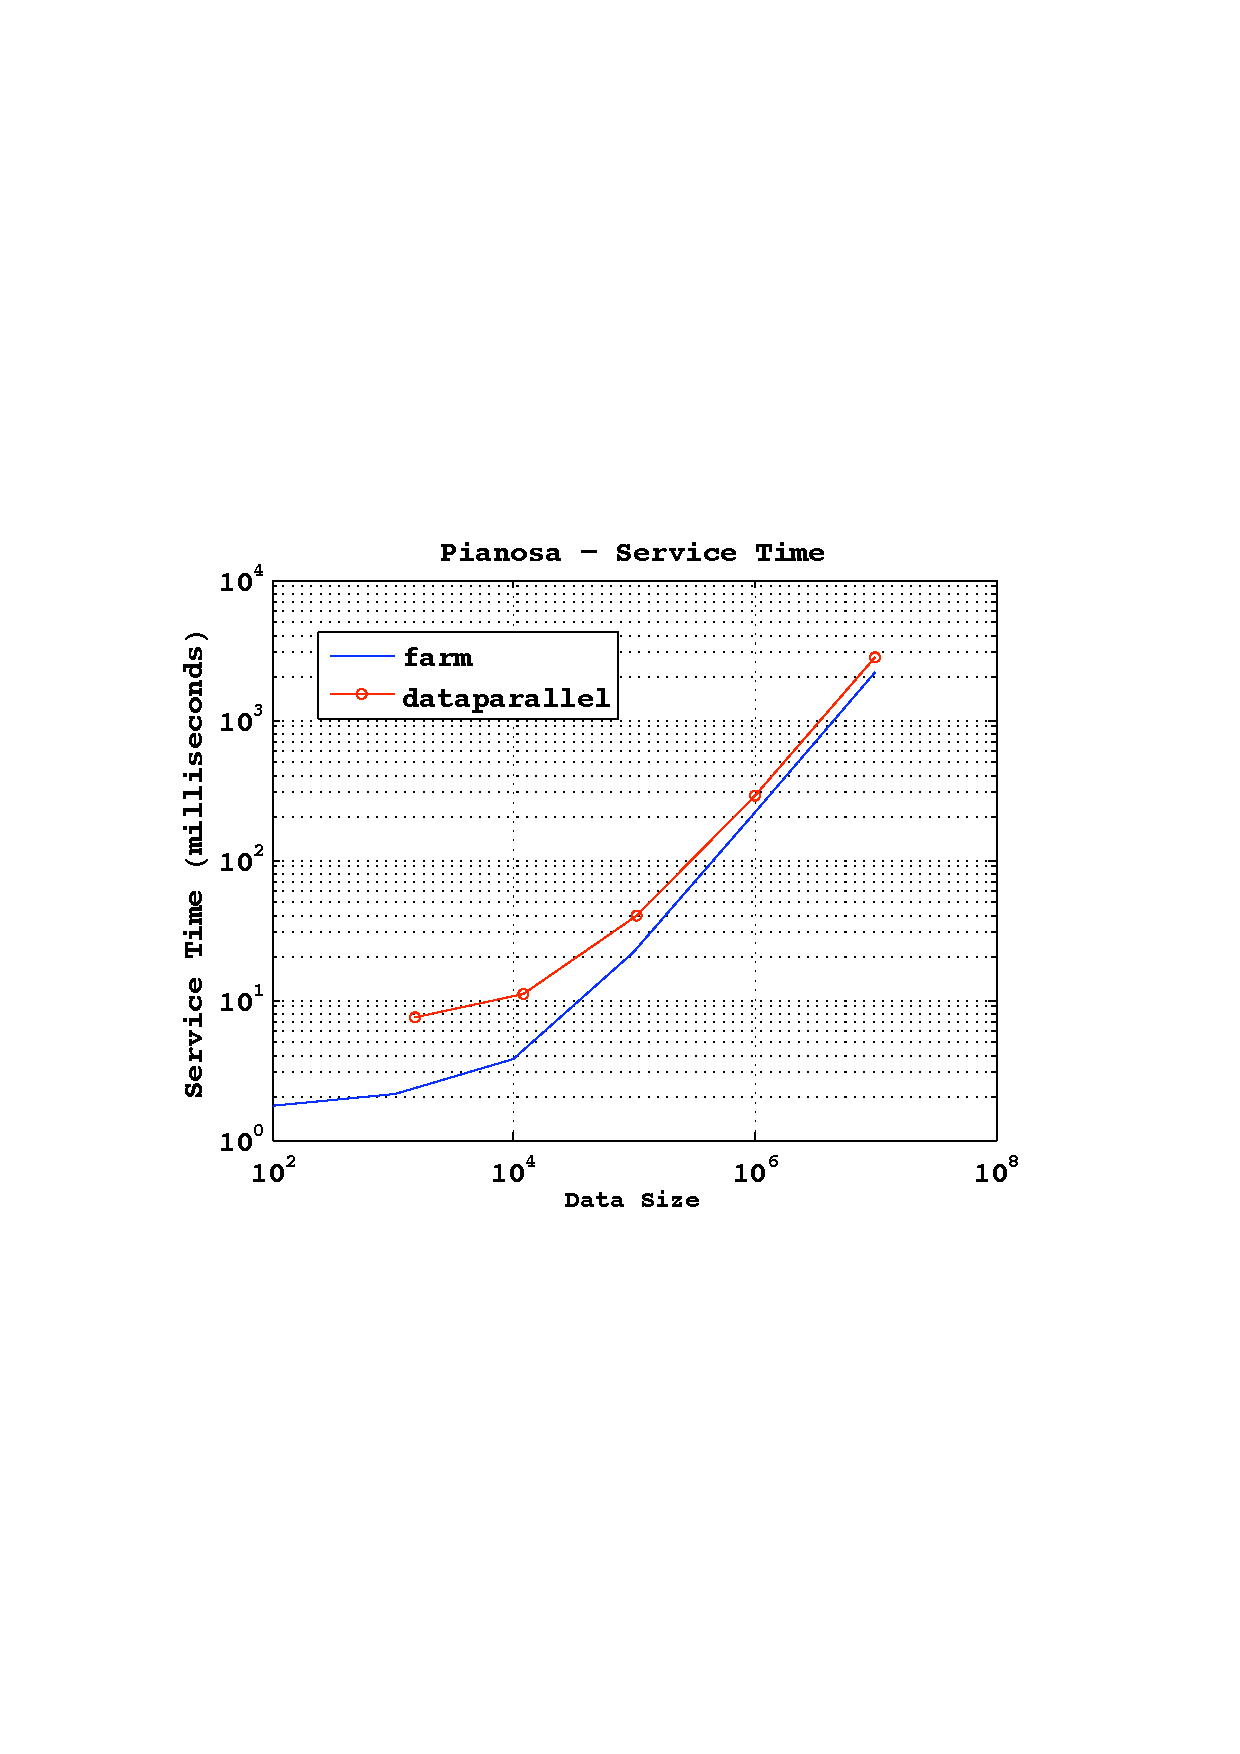
\includegraphics[width=\columnwidth,height=3.5in]{./CHART/pianosa_datascale}%
\label{graf:pianosa_datascale}}
\subfigure[]{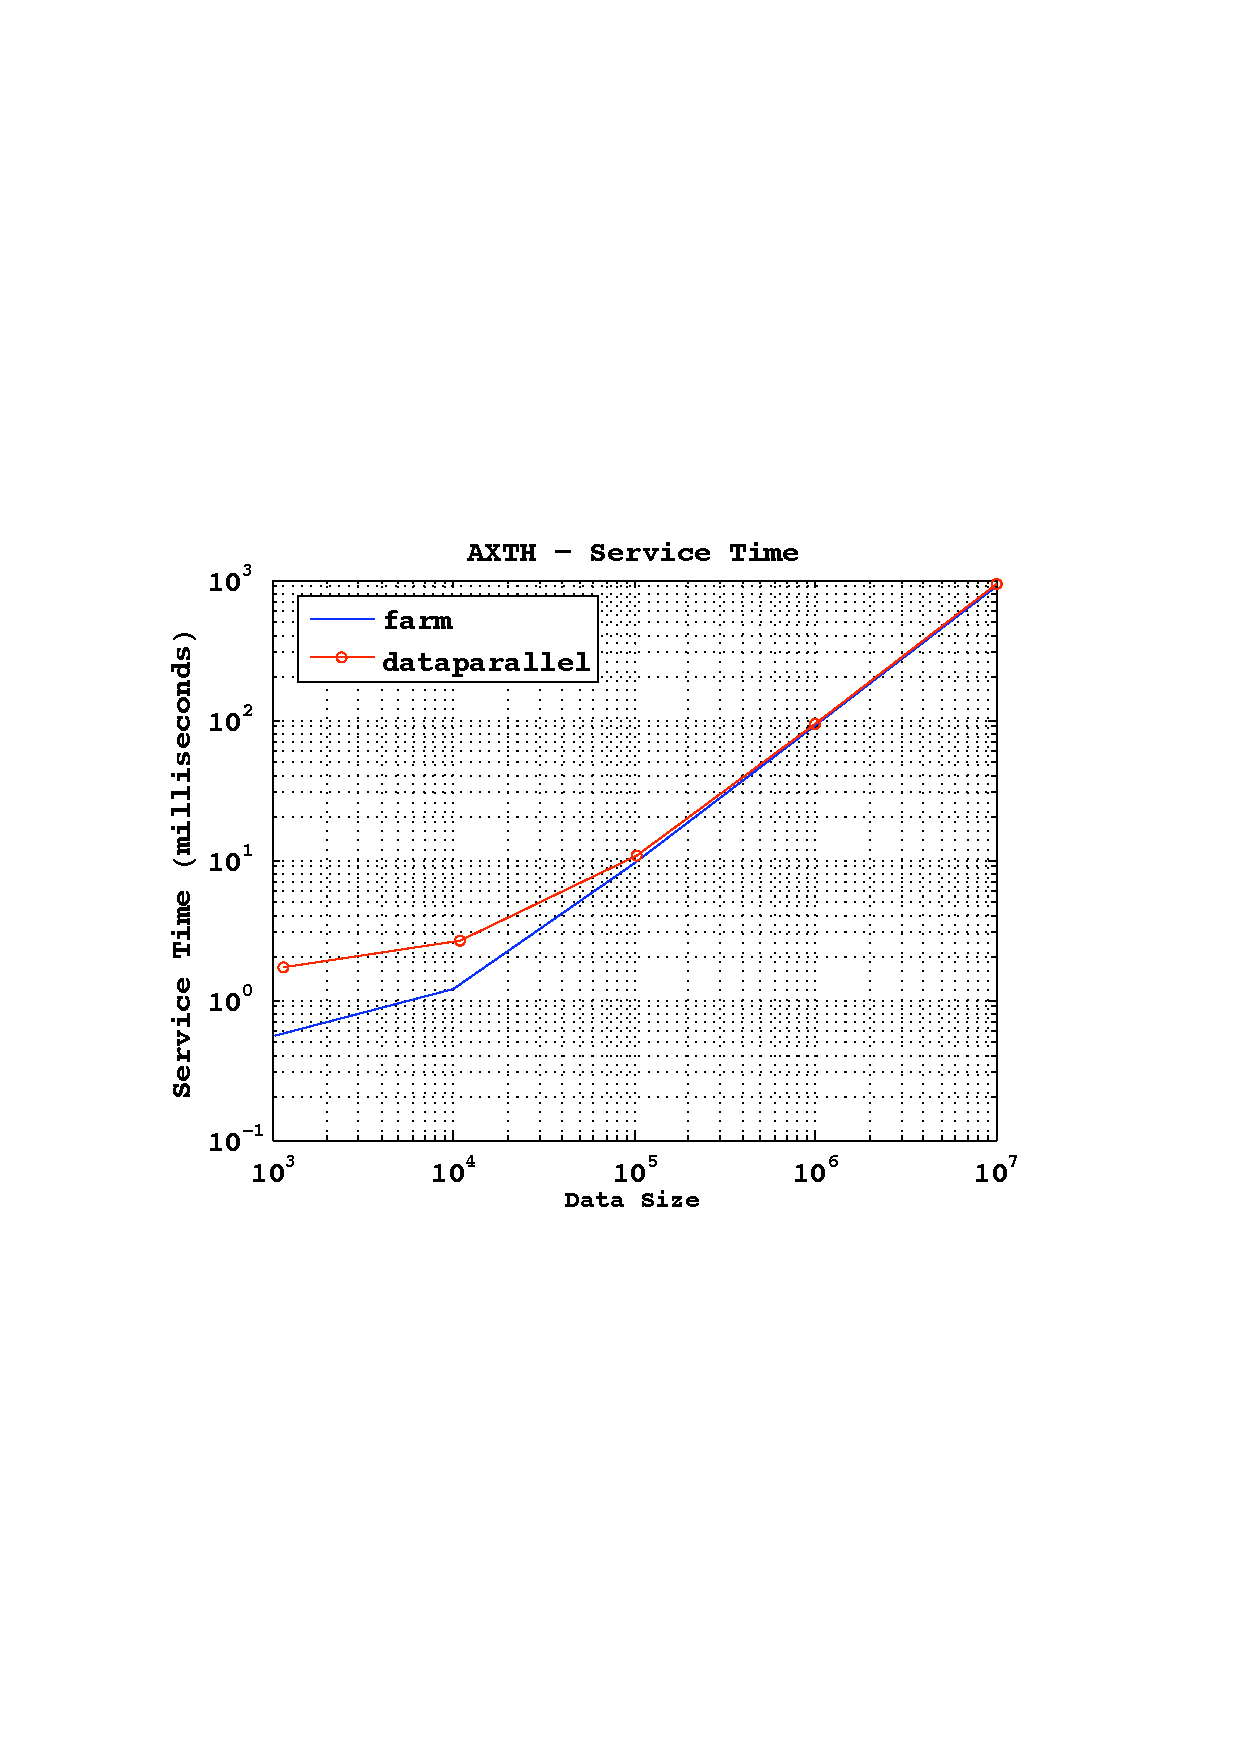
\includegraphics[width=\columnwidth,height=3.5in]{./CHART/axth_datascale}%
\label{graf:axth_datascale}}
\caption{ Service time on the Pianosa cluster of farm and data parallel implementation \ref{graf:time_axth} and relative scalability \ref{graf:pianosa_scala}.  Test is performed on a set of 24 nodes with Intel Pentium III @ 800 Mhz cpu. Images of $10^6$ 8bit pixels.}
\label{chart:pianosa_comm}
\end{figure}

\section{Conclusions}

There are some aspects come out regarding the different choices and the results of the tests that are very interesting and we will discuss them in this section.

The first thing that we can notice from the results of the test \ref{chart:ottavina_farm_1000} is the the fact that, on demand or round robin scheduling, does not affect application performance.
This agrees with the remarks made in Section \ref{farm_cost}.

In the test \ref{chart:ottavina_data_1000} we see that the data parallel scheme can operate in architectures with few nodes with considerably good results.
Instead, this is not possible in the farm solution that we know require at least three nodes. 
For different parallelism degrees of this application, we have a better behaviour of the data parallel scheme. 
This agrees with the remarks made in Section \ref{data_cost} and depends on the memory occupation of the data parallel which is less than the task farm case. 
This effect is noticeable because we are working on a shared memory architecture so data sets of different workers are all stored in the same principal memory.

The test \ref{chart:ottavina_alldata_1000} tells us that the various implementations of data parallel are not particularly different in terms of scalability but they use a number of service processes (zero, one or two processes) that in an architecture with a few nodes can impact the performance.
We also notice that our implementation of scatter and reduce communications have similar performances with respect to \textit{MPI} primitives.
This is mainly due to the really low impact of communication on this architecture as we will see on \ref{graf:Communication}.

Test \ref{chart:ottavina_camera} just shows what happens introducing the external camera module. 
As we can see performance are only slightly affected.



\end{document}